\documentclass[a4paper, 10pt, twoside]{article}

\usepackage[top=1in, bottom=1in, left=1in, right=1in]{geometry}
\usepackage[utf8]{inputenc}
\usepackage[spanish, es-ucroman, es-noquoting]{babel}
\usepackage{setspace}
\usepackage{fancyhdr}
\usepackage{lastpage}
\usepackage{amsmath}
\usepackage{amsfonts}
\usepackage{amsthm}
\usepackage{verbatim}
\usepackage{graphicx}
\usepackage{float}
\usepackage[noend]{algpseudocode}
\usepackage{enumitem} % Provee macro \setlist
\usepackage[toc, page]{appendix}
\usepackage{amsthm}
\usepackage{epstopdf}
\usepackage{amssymb}

%%%%%%%%%% Configuración de amsthm %%%%%%%%%%

\newtheorem{propiedad}{Propiedad}
\newtheorem{demostracion}{Demostración de la Propiedad }

%%%%%%%%%% Configuración de Fancyhdr - Inicio %%%%%%%%%%
\pagestyle{fancy}
\thispagestyle{fancy}
\lhead{Trabajo Práctico 2 · Algoritmos y Estructuras de Datos III}
\rhead{Aboy · Almansi · Canay · Decroix}
\renewcommand{\footrulewidth}{0.4pt}
\cfoot{\thepage /\pageref{LastPage}}

\fancypagestyle{caratula} {
   \fancyhf{}
   \cfoot{\thepage /\pageref{LastPage}}
   \renewcommand{\headrulewidth}{0pt}
   \renewcommand{\footrulewidth}{0pt}
}
%%%%%%%%%% Configuración de Fancyhdr - Fin %%%%%%%%%%


%%%%%%%%%% Configuración de Algorithmic - Inicio %%%%%%%%%%
% Entorno propio para customizar la presentación del pseudocódigo
\newenvironment{pseudo}[1][]{%
    \vspace{0.5em}%
    \begin{algorithmic}%
}
{%
    \end{algorithmic}%
    \vspace{0.5em}%
}

% Valores de verdad
\newcommand{\True}{\textbf{true}}
\newcommand{\False}{\textbf{false}}

% Conectivo 'in' para usar así: \ForAll{$foo$ \In $bar$}
\newcommand{\In}{\textbf{in} }

% Conectivo 'to' para usar así: \For{$i = 1$ \In $n$}
\newcommand{\To}{\textbf{to} }

% Complejidades
\newcommand{\Ode}[1]{\hfill $O(#1)$}
%%%%%%%%%% Configuración de Algorithmic - Fin %%%%%%%%%%


%%%%%%%%%% Miscelánea - Inicio %%%%%%%%%%
% Evita que el documento se estire verticalmente para ocupar el espacio vacío
% en cada página.
\raggedbottom

% Deshabilita sangría en la primer línea de un párrafo.
\setlength{\parindent}{0em}

% Separación entre párrafos.
\setlength{\parskip}{0.5em}

% Separación entre elementos de listas.
\setlist{itemsep=0.5em}

% Asigna la traducción de la palabra 'Appendices'.
\renewcommand{\appendixtocname}{Apéndices}
\renewcommand{\appendixpagename}{Apéndices}
%%%%%%%%%% Miscelánea - Fin %%%%%%%%%%


%%%%%%%%%% Gráficos - Inicio %%%%%%%%%%
% Macro para incluir tres gráficos (dentro de una figura) de manera que
% entren todos en una sola página.
\newcommand{\tresgraficos}[3]{
    \newcommand{\separacion}{-2.2em}
    \vspace{\separacion}
    \include{#1}
    \vspace{\separacion}
    \include{#2}
    \vspace{\separacion}
    \include{#3}
}
%%%%%%%%%% Gráficos - Fin %%%%%%%%%%


\begin{document}


%%%%%%%%%%%%%%%%%%%%%%%%%%%%%%%%%%%%%%%%%%%%%%%%%%%%%%%%%%%%%%%%%%%%%%%%%%%%%%%
%% Carátula                                                                  %%
%%%%%%%%%%%%%%%%%%%%%%%%%%%%%%%%%%%%%%%%%%%%%%%%%%%%%%%%%%%%%%%%%%%%%%%%%%%%%%%

\thispagestyle{caratula}

\begin{center}


\includegraphics[width=0.6\textwidth]{./img/DC.jpg} 
% 
\includegraphics[width=0.3\textwidth]{./img/UBA.jpg} 
\hfill

\vspace{2cm}

\begin{Huge}
Trabajo Práctico 2
\end{Huge}

\vspace{0.5cm}

\begin{Large}
Algoritmos y Estructuras de Datos III
\end{Large}

\vspace{1cm}

\begin{Large}
Primer Cuatrimestre de 2014
\end{Large}

\vspace{2cm}

\begin{tabular}{|c|c|c|}
\hline
Alumno & LU & E-mail\\
\hline
Aboy Solanes, Santiago    & 175/12 & santiaboy2@hotmail.com\\
Almansi, Emilio Guido     & 674/12 & ealmansi@gmail.com\\
Canay, Federico José      & 250/12 & fcanay@hotmail.com\\
Decroix, Facundo Nicolás  & 842/11 & fndecroix92@hotmail.com\\
\hline
\end{tabular}

\vspace{4cm}

Departamento de Computación,\\
Facultad de Ciencias Exactas y Naturales,\\
Universidad de Buenos Aires

\end{center}

\newpage


%%%%%%%%%%%%%%%%%%%%%%%%%%%%%%%%%%%%%%%%%%%%%%%%%%%%%%%%%%%%%%%%%%%%%%%%%%%%%%%
%% Índice                                                                    %%
%%%%%%%%%%%%%%%%%%%%%%%%%%%%%%%%%%%%%%%%%%%%%%%%%%%%%%%%%%%%%%%%%%%%%%%%%%%%%%%

\tableofcontents

\newpage


%%%%%%%%%%%%%%%%%%%%%%%%%%%%%%%%%%%%%%%%%%%%%%%%%%%%%%%%%%%%%%%%%%%%%%%%%%%%%%%
%% Introducción                                                              %%
%%%%%%%%%%%%%%%%%%%%%%%%%%%%%%%%%%%%%%%%%%%%%%%%%%%%%%%%%%%%%%%%%%%%%%%%%%%%%%%

\section{Introducción}
El objetivo de este informe es describir, desarrollar y presentar una solución algorítmica a tres problemas de maximización/minimización u optimización. Por otro lado, demostraremos la correctitud de las soluciones propuestas, y que su complejidad temporal cumple los requerimientos pedidos. Realizamos diversos experimentos que permiten verificar la correctitud, así como también realizamos experimentaciones computacionales para medir la performance de la implementación de nuestra solución. Los resultados obtenidos y la discusión de los mismos se encuentran en sus secciones correspondientes.

El código fuente de las soluciones se encuentran en su totalidad en la carpeta \emph{src}, mientras que sus secciones más relevantes se pueden leer en los apéndices de este informe.

\section{Consideraciones generales}
\subsection{Lenguaje de implementación}

Para implementar las soluciones algorítmicas desarrolladas en cada problema utilizamos el lenguaje C++, el cual presenta una serie de características muy convenientes. Este lenguaje es imperativo, al igual que el lenguaje de pseudocódigo utilizado para describir las soluciones y probar su correctitud. Adicionalmente, el mismo posee librerías estándar muy completas, versátiles y bien documentadas, lo cual permite abstraer el manejo de memoria, la implementación de estructuras de datos y algoritmos de uso frecuente, y provee mecanismos para realizar mediciones de tiempo de manera fidedigna.

\subsection{Algoritmo de ordenamiento}

En las implementaciones desarrollados para resolver los problemas planteados, utilizamos la función \emph{sort} de la Standard Template Library (STL). Para que la complejidad temporal de las soluciones se condiga con el análisis teórico, es necesario verificar que dicha función tenga efectivamente una complejidad temporal $O(n * log(n))$.

En la página de documentación oficial cppreference\footnote{http://en.cppreference.com/w/cpp/algorithm/sort}, se observa que a partir del standard C+11 de C++, la complejidad requerida para std::sort es de $O(n*log (n))$ 
comparaciones, y a lo sumo $O(n * log(n))$ swaps. Como utilizamos contenedores de acceso aleatorio en tiempo constante para desarrollar las soluciones, las operaciones de comparación y swap son $O(1)$. Por esto, efectivamente las rutinas de ordenamiento utilizadas tienen una complejidad de $O(n * log(n))$ operaciones.

% Con sólo esta informacion no podemos asegurar que el algoritmo en su totalidad tenga una complejidad temporal de $O(n*log (n))$  operaciones, por lo que buscamos que hace el algoritmo \emph{std::sort} revisando el código de \emph{algorithm.h}.

% esto no esta bien
 %Encontramos que, para casos con cantidad de elementos a ordenar menor a 64, hace un sort especial (el cual no nos interesa ya que queremos evaluar lo que pasa para $n$ grande). 

%esto depende exclusivamente de la implementacion que estás usando, y no del standard!
 %En casos mas grandes, realiza \emph{IntroSort}. \emph{IntroSort} intenta ordenar usando \emph{QuickSort}, si no lo resuelve en $n*log (n)$ pasos, usa HeapSort para garantizar $O(n*log (n))$ comparaciones.


\subsection{Mediciones de performance}
\label{consideraciones-mediciones}

Para llevar a cabo mediciones de performance sobre las implementaciones desarrolladas, medimos el tiempo consumido para resolver instancias de sucesivos tamaños en función de un parámetro a definir según el caso. Procuramos medir exclusivamente el tiempo consumido por la etapa de resolución, ignorando tareas adicionales propias al proceso como, por ejemplo, la generación de la instancia a ser resuelta.

La función del sistema que se escogió para medir intervalos de tiempo es la siguiente:

\begin{verbatim}
  int clock_gettime(clockid_t clk_id, struct timespec *tp);
\end{verbatim}

de la librería \emph{time.h}. La misma nos permite realizar mediciones de alta resolución, específicas al tiempo de ejecución del proceso que la invoca (y no al sistema en su totalidad), configurando el parámetro clk\_id con el valor CLOCK\_PROCESS\_CPUTIME\_ID\footnote{http://linux.die.net/man/3/clock\_gettime}.

Por otro lado, dado que la medición de tiempos en un sistema operativo activo introduce inherentemente un cierto nivel de ruido, cada medición se realizó múltiples veces. Una vez obtenidos los distintos valores para una misma medición (es decir, para diferentes instancias del mismo tamaño), registramos como valor definitivo la mediana de la serie de valores. Escogimos este criterio en vez de, por ejemplo, tomar la media, ya que utilizar la mediana es menos suceptible a la presencia de valores atípicos o \emph{outliers}.

\newpage


%%%%%%%%%%%%%%%%%%%%%%%%%%%%%%%%%%%%%%%%%%%%%%%%%%%%%%%%%%%%%%%%%%%%%%%%%%%%%%%
%% Problema 1: Camiones sospechosos                                          %%
%%%%%%%%%%%%%%%%%%%%%%%%%%%%%%%%%%%%%%%%%%%%%%%%%%%%%%%%%%%%%%%%%%%%%%%%%%%%%%%

\section{Problema 1: Robanúmeros}

\subsection{Descripción del problema}
\label{problema1-descripcion}
Este problema trata de un juego de cartas llamado \emph{Robanúmeros}. El mismo es un juego para dos jugadores. Al empezar el juego se cuenta con una secuencia de cartas, todas ellas boca arriba, cada carta tiene un valor numérico entero (puede ser positivo o negativo). Este juego se juega por turnos de forma alterna y en cada turno un jugador debe elegir un extremo de la secuencia de cartas y robar una cantidad de las mismas empezando desde ese extremo. Por ejemplo supongamos que la secuencia de cartas es la dada en la siguiente tabla:

\begin{tabular}{|c|c|c|c|c|}
\hline
2 & -3 & 7 & 8 & -10 \\
\hline
\end{tabular}

Dada esta secuencia, el primer jugador en jugar puede, por ejemplo, elegir el extremo derecho y robar 3 cartas, quedándose así con -10, 8 y 7. También podría elegir 4 cartas por el lado izquierdo y de esta forma se quedaría con 2, -3, 7 y 8. Sin embargo, el jugador no puede robar 2, -3 y 8, o -10, y -3.

En cada turno el jugador debe robar al menos una carta y al no quedar más, el jugador que obtenga el número más alto al sumar los valores de todas las cartas que robó es el ganador.

En este problema debemos diseñar un algoritmo que juegue a este juego de manera óptima. Este algoritmo debe estar pensado para jugar contra otro jugador que también juegue de forma óptima. La definición de que un jugador juegue de manera óptima significa que la diferencia de puntos obtenida a su favor sea la mayor diferencia que se puede obtener frente a un oponente que también juega de la misma forma ante cada situación que se le deje.

El algoritmo debe tener una complejidad temporal de peor caso de $O(n^3)$ donde $n$ es la cantidad de cartas en la secuencia inicial.

\subsubsection{Ejemplos y observaciones}



\subsection{Desarrollo de la solución}
\label{problema1-desarrollo}
Modelamos este problema de la siguiente manera:

$\bullet$ Un pueblo es un par ordenado (x,y).

$\bullet$ Una tubería es un par no ordenado de pueblos.

$\bullet$ Un conjunto de V pueblos y otro E de tuberías puede ser considerado un grafo, cuyo conjunto de nodos es V y su conjunto de aristas es E.

$\bullet$ El peso asociado a una arista (tubería) es igual a la distancia euclidiana entre los extremos (pueblos).

$\bullet$ Una central es un pueblo.

$\bullet$ Dado V un conjunto de pueblos y k la cantidad de centrales de gas, una solución es un conjunto $C \subseteq V$ de k pueblos y un grafo B(V,E), sea E el conjunto de tuberías que decidimos colocar para conectar los pueblos. Por ejemplo, si queremos conectar al pueblo 'a' y al pueblo 'b', agregamos al conjunto E la arista ('a','b'). El subonjunto C representa a los pueblos donde elegimos poner las centrales.  

$\bullet$ Dada una solución conformada por C y B(V,E), un pueblo $v \in V$ esta provisto de gas si existe un camino en B entre éste y un pueblo $c \in C$ ya que estos pueblos son los que tienen central distribuidora.

$\bullet$ Dada una solución C, B(V,E) decimos que la misma es factible si $(\forall v \in V)(\exists c \in C) \exists$ un camino entre v y c en B. 

$\bullet$ Queremos encontrar el C , B(V,E) tal que sea una solución óptima, minimizando la máxima arista.

Consideramos una solución, si cumple la aridad pedida. Una solución factible si cumple cierta condicion además de la aridad. Una solución optima es quien maximiza/minimiza cierta funcion entre todas las soluciones factibles, en este caso se busca minimizar la máxima arista.

Supongamos que tenemos el conjunto V que contiene a todos los pueblos. Sea G(V,E) un grafo completo donde el peso de las aristas es igual a la distancia euclidiana entre los pueblos. Para encontrar la solución óptima vamos a encontrar B(V,E) un bosque generador mínimo con k componentes conexas de G y C un conjunto que  contenga un pueblo de cada una de las componentes conexas de B.

Definiendo un bosque generador mínimo con k componentes conexas de G, como un grafo que cumple las siguientes condiciones:

$\bullet$Es un subgrafo generador de G. 

$\bullet$Es un bosque de k componentes conexas.

$\bullet$ Entre todos los subgrafos generador de G de k componentes conexas tiene la mínima suma de aristas.

Ahora presentaremos una idea de por este modelo efectivamente resuelve el problema. Luego lo vamos a demostrar formalmente. 

$\bullet$ Un bosque de k componentes conexas generador mínimo también minimiza la máxima arista.

$\bullet$ Dada una solución C, B(V,E), es factible $\Longleftrightarrow$ $(\forall D$ componente conexa de $B)((\exists v \in D) v \in C)$.  

$\bullet$ Dada una solución con i componentes conexas (siendo i $<$ k), existe una solución mejor o igual con i+1 componentes conexas.

Vamos a suponer que k $\leq$ n, ya que en el caso contrario la solución es trivial. Cada pueblo tiene una central y no se necesitan construir ninguna tubería.

\subsection{Complejidad temporal}
\label{problema1-complejidad}
En la figura que muestra el pseudocódigo de nuestro algoritmo situada arriba podemos ver que la complejidad de este algoritmo se representa con esta cuenta:

$O(n) + 2*O(1) + n*(2*O(1) + n*(2*O(1) +O(n) + 6*O(1)) + O(n)$

Por álgebra de órdenes esto se puede reducir a:

$O(2n+2) + n*(O(2) + n*(O(2) + O(n) + O (6)))$

$O(n) + n*(O(1) + n*(O(n+1)))$

$O(n) + n*(O(1) + O(n^2+n))$

$O(n) + n*(O(n^2 +n +1))$

$O(n) + n*O(n^2)$

$O(n^3+n)$

$O(n^3)$

Entonces podemos decir que la complejidad de nuestro algoritmo es $O(n^3)$, pero primero tenemos que demostrar que los algoritmos $escribirSalida$ y $buscarMinimo$ realmente tienen una complejidad lineal.

El algoritmo de $buscarMinimo$ es el siguiente

\begin{center}
 \begin{figure}[H]
  \begin{pseudo}
   \Procedure{buscarMinimo}{opt,i,j,iSiguiente,jSiguiente,minCantPuntos}
    \State $k \leftarrow 1$\Ode{1}
    \While{$k \leq j-1$} \hfill $n*O(1)$
      \If{$opt[i+k][j].cantPuntos < minCantPuntos$ }\Ode{1}
	\State $iSiguiente \leftarrow i+k$\Ode{1}
	\State $jSiguiente \leftarrow j$\Ode{1}
	\State $minCantPuntos \leftarrow opt[i+k][j].cantPuntos$\Ode{1}
      \EndIf
      \If{$opt[i][j-k].cantPuntos < mincantPuntos$}\Ode{1}
	\State $iSiguiente \leftarrow i$\Ode{1}
	\State $jSiguiente \leftarrow j-k$\Ode{1}
	\State $mincantPuntos \leftarrow opt[i][j-k].cantPuntos$\Ode{1}
      \EndIf
    \EndWhile
   \EndProcedure
  \end{pseudo}

 \end{figure}

\end{center}

La complejidad del algoritmo es:

$O(1) + n*(8*O(1))$

Por álgebra de órdenes:

$O(1) + O(8*n)$

$O(n)$

Ahora veamos que el algoritmo $escribirSalida$ también tiene complejidad lineal:

%Continuará


\label{problema1-demostracion}
\subsection{Demostración de correctitud}
Para demostrar que nuestra solución resuelve el problema propuesto tenemos que demostrar dos cosas. La primera es que la función recursiva que nosotros propusimos realmente determina los movimientos óptimos para realizar y la segunda es que la matriz que usamos para guardar las subsoluciones es completada correctamente.

Primero vamos a demostrar que la función recursiva determina las jugadas óptimas del juego. 

Para empezar recordemos lo que lo que el problema pide es jugar de una forma que maximice tu puntuación. Como al finalizar el juego no pueden quedar cartas sin robar, la suma de los valores de todas las cartas va a estar distribuida entre el jugador uno y el jugador dos, de esta forma:

$\sum_{i=0}^{n} c_i = \sum_{j \in A} c_j + \sum_{k \in B} c_k$

Donde A es el conjunto de cartas que robó el jugador uno y B es el conjunto de cartas que robó el jugador dos.

Por lo tanto mientras más chico sea el valor de la suma de los valores del conjunto B, el valor del conjunto A va a crecer, y viceversa, ya que se da la siguiente igualdad:

$\sum_{i=0}^{n} c_i  - \sum_{j \in B} c_j= \sum_{k \in A} c_k$

Supongamos que somos el jugador uno. Lo que el problema pide es que juguemos de forma óptima, por lo tanto debemos maximizar nuestra puntuación. Maximizar nuestra puntuación es maximizar el valor de la suma de los elementos de A, y  por lo que acabamos de ver esto es lo mismo que minimizar la suma de los elementos de B, que representa la puntuación del jugador dos.

Recordemos que nuestra función recursiva es la siguiente:

$opt(i,i) = c_i$ \\
$opt(i,j) = \sum cartas - min(opt(i+1, j), ..., opt(j,j), opt(i, j-1), ... ,opt(i,i), 0)$

Por lo dicho anteriormente demostrar que nuestra función resuelve el problema es lo mismo que demostrar que nuestra función minimiza el puntaje del jugador contrario.

Vamos a demostrar esto por inducción en las cartas restantes, que en este caso son $j-i+1$. La propiedad que queremos demostrar es la siguiente:

$P(i,j) : (\forall i,j, 0 \leq i \leq j < n)opt(i,j)$ maximiza nuestro puntaje para las cartas desde $c_i$ hasta $c_j$

Primero analicemos el caso base:

$opt(i,i) = c_i$

Queremos ver que se cumple $P(i,i)$.

Este caso significa que sólo queda una carta. Como el juego nos obliga a, de ser posible, robar al menos una carta por turno, la única opción posible es robar esta carta. Como es la última opción, también es la opción óptima, por lo tanto se cumple $P(i,i)$.

Ahora analicemos el caso recursivo:

$opt(i,j) = \sum cartas - min(opt(i+1, j), ..., opt(j,j), opt(i, j-1), ... ,opt(i,i), 0)$

Tenemos que realizar el paso inductivo, esto significa que tenemos que probar que $P(i,j)$ seguro vale si vale $P(i',j')$ para todas las subsecuencias de cartas que $opt(i,j)$ utiliza, osea, para probar $P(i,j)$ queremos ver que:

$[(\forall i',j',(( i < i' \wedge j = j') \vee (i' = i \wedge j' < j))) P(i',j')]  \implies P(i,j)$

\textbf{HI:} $((\forall i',j',(( i < i' \wedge j = j') \vee (i' = i \wedge j' < j))) P(i',j'))$

Para demostrar esto vamos a dar como válida la hipótesis inductiva y a partir de eso probar que vale $P(i,j)$.

En este caso quedan $j-i+1$ cartas, tenemos que demostrar que $opt(i,j)$ toma la decisión que minimiza el puntaje del jugador contrario. Como el problema nos dice que tenemos que asumir que el jugador contrario también juega de forma óptima, entonces su puntaje también estará determinado por la función $opt$.

Lo que la función debe determinar es, de las posibles instancias del juego que se pueden generar luego de jugar nuestro turno, la que minimiza la función de $opt$ ya que el puntaje del jugador contrario será el resultado de aplicar $opt$ a la instancia que quede. Y por hipótesis inductiva sabemos que al aplicar $opt$ a dicha instancia se obtendrá un resultado óptimo.

Como sólo se pueden robar cartas de uno de los dos extremos las posibles instancias son las siguientes: Si se roba una carta comenzando de la izquierda la instancia generada será de $(i+1,j)$, si se roban 2, de $(i+2,j)$ y se se roban $j-i$, de $(j,j)$. De esta misma forma si se roba una carta empezando de la derecha quedará una instancia de $(i,j-1)$ y si se roban $j-i$ cartas, la instancia sera de $(i,i)$.

Pero queda una instancia más por analizar, la de levantar todas las cartas posibles (no importa de cual extremo). En ese caso se generará una instancia $(0,0)$.

Por lo tanto el mínimo que debemos hallar es el siguiente:

$min(opt(i+1,j), ... , opt(j,j), opt(i,j-1), ... , opt(i,i), 0)$

Y la puntuación óptima se determina por la cuenta:

$\sum cartas - min(opt(i+1,j), ... , opt(j,j), opt(i,j-1), ... , opt(i,i), 0)$

Por lo tanto, si asumimos que se cumple nuestra hipótesis inductiva, nuestra función $opt$ minimiza el puntaje del jugador contrario. Osea que realmente determina nuestra puntuación óptima y el movimiento a realizar para obtenerla, que es lo que el problema pide.

Lo que queda mostrar es que completamos la matriz de forma correcta. Como cada casilla de la matriz es un subproblema y para resolver cada subproblema usamos subproblemas mas chicos, tenemos que mostrar que a la hora de completar una casilla siempre tenemos completas las casillas de los subproblemas que se necesitan.

La matriz, tal y como dijimos en el desarrollo, se completa de arriba a abajo y de izquierda a derecha.

Entonces, supongamos que queremos llenar la casilla $opt[i][j]$. Como la matriz se llena de abajo hacia arriba, a la hora de llenar esta casilla ya van a estar llenas las casillas $opt[i][j']$ donde $j < j'$. Y como la matriz se llena de izquierda a derecha, a la hora de completar esta casilla ya van a estar completas las casillas $opt[i'][j]$, donde $i' < i$.

Además, como dijimos en el desarrollo para llenar una casilla $opt[i][j]$ se necesita observar los valores de las casillas que están a la izquierda de la ésta y las que están abajo. Como se muestra en la Figura 1.

Osea que las casillas necesarias son $opt[i'][j]$, donde $i' < i$ y $opt[i][j']$ donde $j < j'$. Estas son las mismas casillas que ya dijimos que iban a estar completas a la hora de completar $opt[i][j]$. Por lo tanto al completar $opt[i][j]$ casilla van a estar previamente completadas las casillas necesarias para hacerlo, por lo tanto nuestra matriz se llena correctamente.

\subsection{Experimentación}
\label{problema1-experimentacion}
En esta sección, vamos a comprobar empíricamente que nuestro algoritmo tiene una complejidad temporal cúbica respecto de n, y lineal respecto de k.

En un primer caso, utilizamos instancias donde cada casillero tiene una potencia en función de n: p(n) = $n/5$. Una vez más, utilizamos k distintos entre sí, pero fijos en cada caso. Probamos con distintos $n$ y obtuvimos el resultado que se puede observar en las figuras debajo.

\begin{figure}[H]
  \begin{minipage}{0.5\linewidth}
    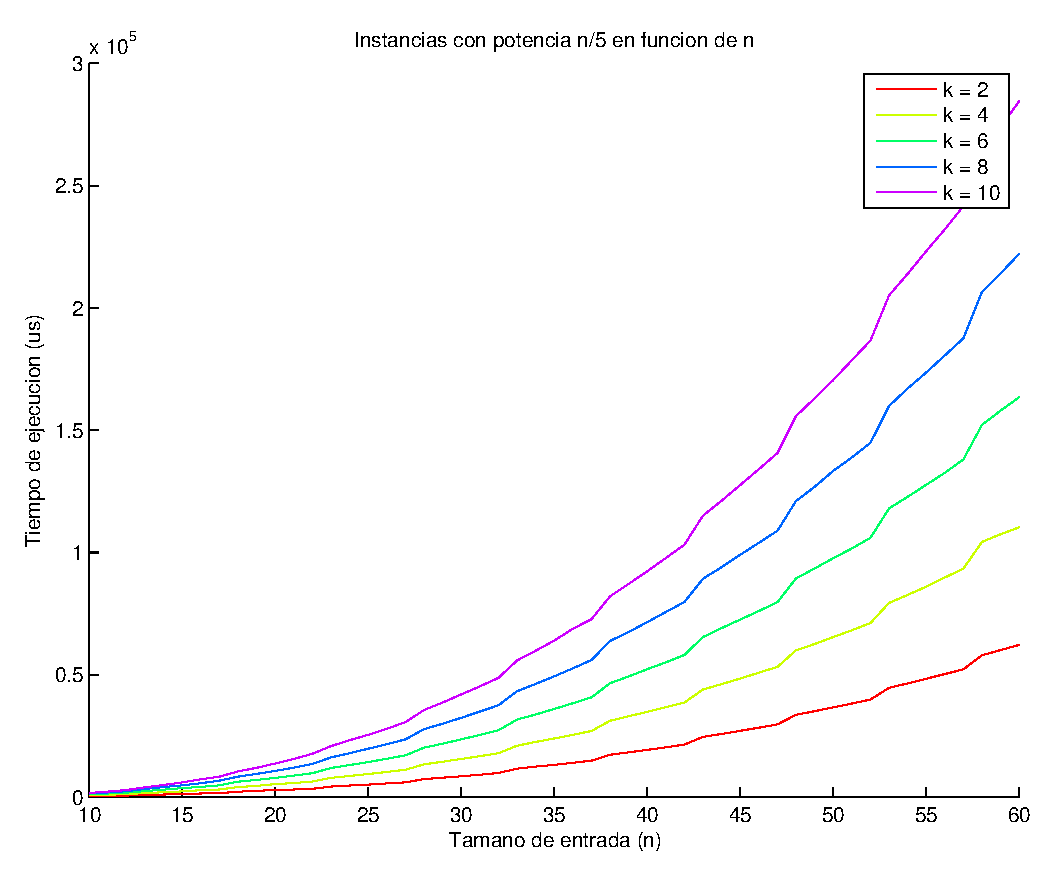
\includegraphics[width=\linewidth]{img/problema3/instancia_p_20p_varios_k.eps}
    \caption{Tiempo de ejecución, p(n) = $n/5$}\label{fig:problema3-k-20}
  \end{minipage}
  \hfill
  \begin{minipage}{0.5\linewidth}
    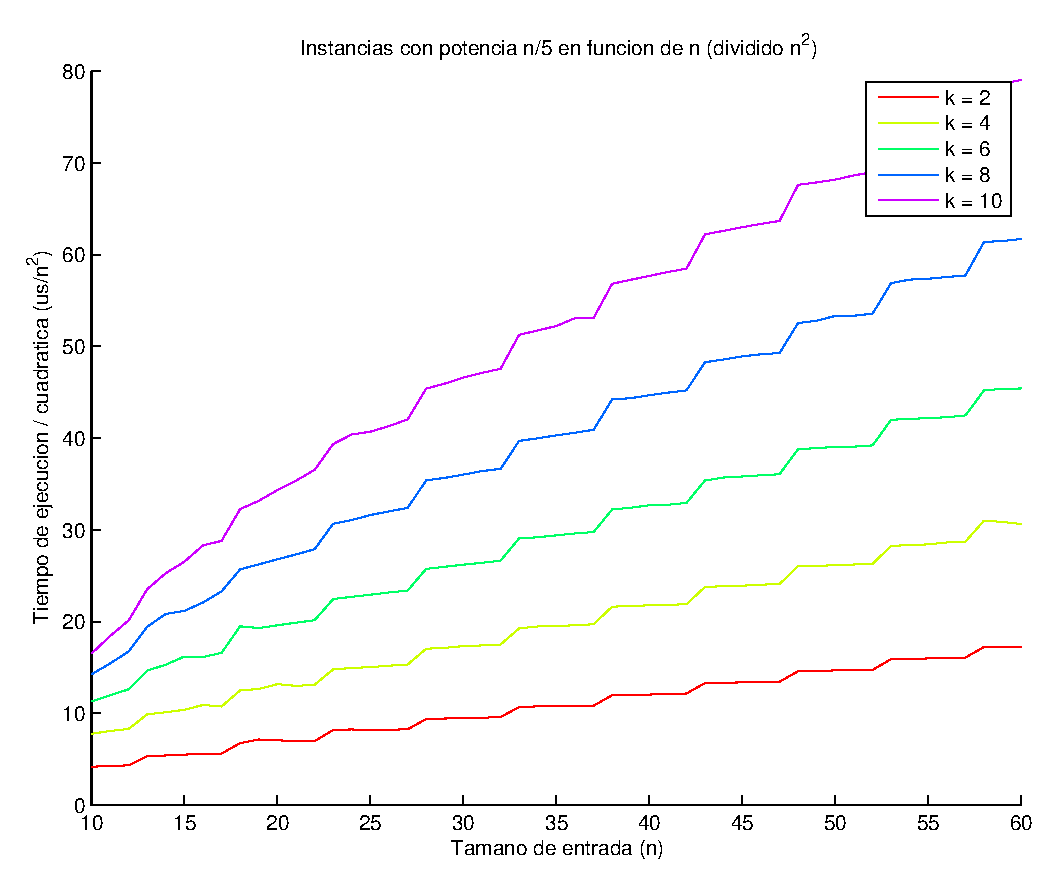
\includegraphics[width=\linewidth]{img/problema3/instancia_p_20p_varios_k_div_n2.eps}
    \caption{Idem, dividido por $n^2$}\label{fig:problema3-k-n2-20}
  \end{minipage}	
\end{figure}

En la figura \ref{fig:problema3-k-20} no podemos notar la complejidad temporal de la función. Por esto, dividimos por $n^2$ y plasmamos ese resultado en la figura \ref{fig:problema3-k-n2-20}. Sin embargo, en esta última figura tampoco podemos ver claramente la complejidad temporal. Por esta razón, decidimos analizar los ``saltos'' que pega la función. Luego de experimentación y búsqueda llegamos a la conclusión que esos saltos se relacionan con el cambio de potencia de los resortes. Por ejemplo entre para n entre 10 y 15 las potencias son de la siguiente manera: 2,2,2,3,3,3. Esto se debe a que 12/5 = 2.4 (y lo redondea para abajo) y 13/5 = 2.6 (que se redondea para arriba).

Una vez que entendimos estos saltos, llegamos a la conclusión que si tomamos los puntos donde pega los saltos la función y trazamos una recta $r$, la recta correspondiente al tiempo de ejecución va a tener una pendiente menor o igual a la pendiente de la recta $r$. Es decir, que comprobamos que por más que la potencia dependa del n la complejidad temporal también es lineal respecto de $T(N)/n^2$ que es lo mismo que decir que es cúbica respecto de n.

Finalmente, decidimos hacer un experimento más: utilizamos n distintos entre sí (pero fijos en cada caso) y variar el k. Una vez más p depende de n con la misma función anteriormente usada.

\begin{figure}[H]
  \begin{minipage}{0.5\linewidth}
    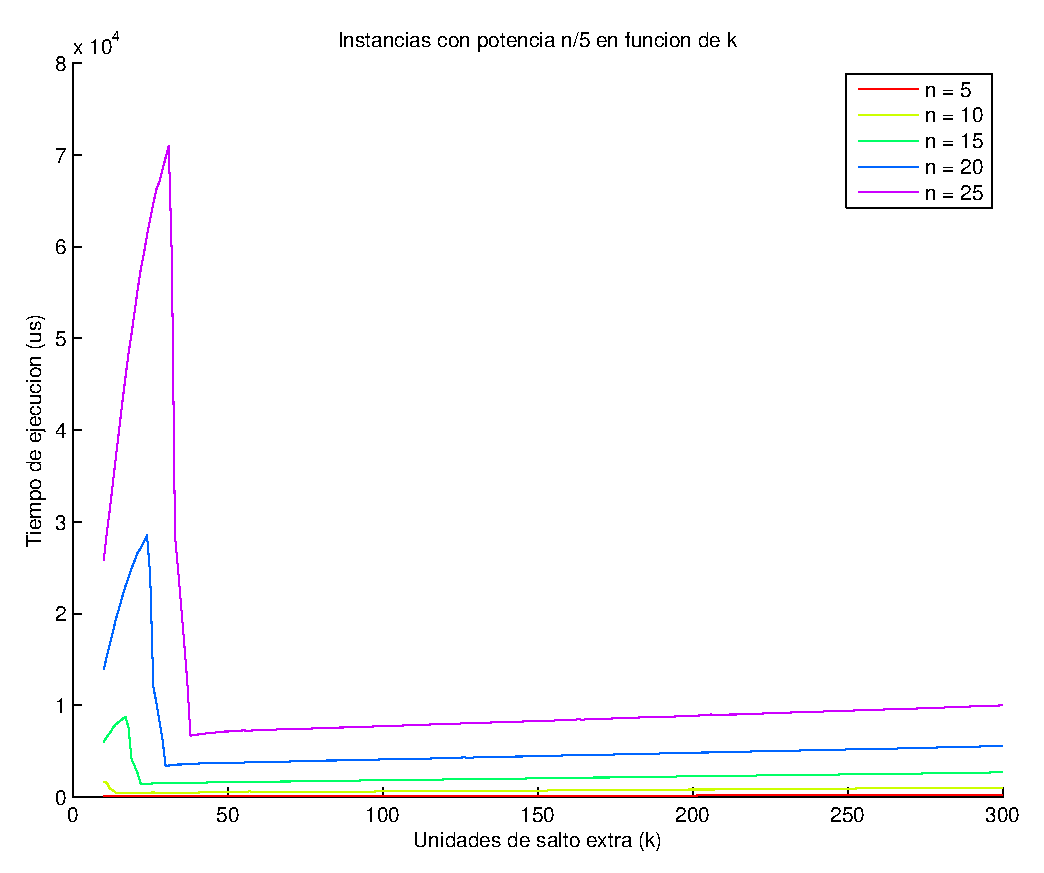
\includegraphics[width=\linewidth]{img/problema3/instancia_p_20p_varios_n.eps}
    \caption{Tiempo de ejecución, p(n) = $n/5$}\label{fig:problema3-n-20}
  \end{minipage}
  \hfill
  \begin{minipage}{0.5\linewidth}
    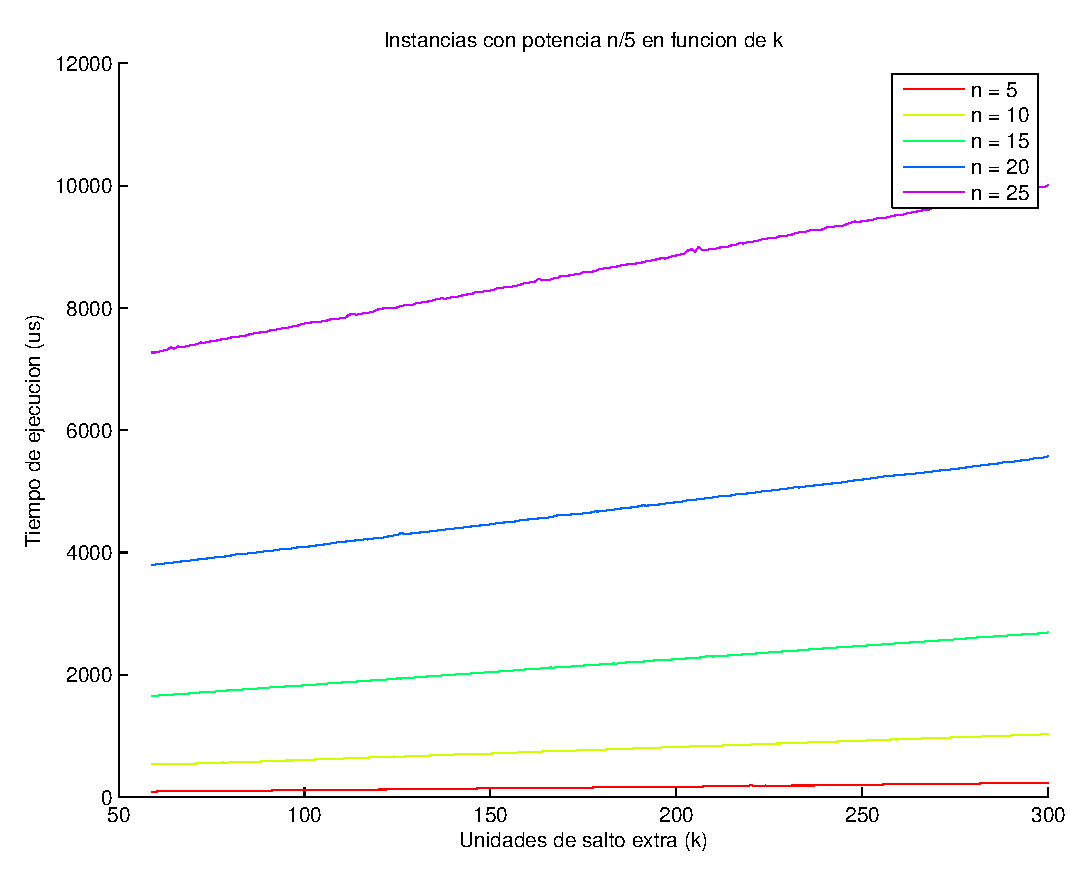
\includegraphics[width=\linewidth]{img/problema3/instancia_p_20p_varios_n_zoom.eps}
    \caption{Idem, con \emph{zoom}}\label{fig:problema3-n-n2-20}
  \end{minipage}
\end{figure}

En estos casos, una vez más podemos observar que cuando $k \geq 2*(n-1-p)$ resolver el problema es trivial. En estas figuras, está representado por la caída del tiempo de ejecución a partir de este punto. Cabe aclarar que si bien resolver el problema es trivial, al crecer el n cuesta más crear la matriz3D ya que la misma es más grande. En estos casos, la complejidad temporal de nuestro algoritmo es lineal respecto de k.

Para poder ver mejor esto último, realizamos \emph{zoom} a la figura a partir del momento de la caída, lo cual lo podemos ver en la figura \ref{fig:problema3-n-n2-20}. En esta figura, se ve claramente que la complejidad temporal de nuestro algoritmo es lineal respecto de k.

%TODO les parece poner un apendice con mas graficos o lo dejamos asi?

\subsection{Conclusión}
\label{problema1-resultados}
Si bien el problema tratado pareciera a primera vista admitir una solución en la forma de programación dinámica, el hecho de tener un recurso agotable en consideración no permite aplicar el principio de optimalidad. Es decir, es posible que en un camino óptimo se llegue a un casillero intermedio de forma subóptima (posiblemente para ahorrar unidades de salto extra).

De todas formas, el problema puede ser resuelto eficientemente una vez que se modela apropiadamente mediante grafos, utilizando el algorítmo de búsqueda BFS. En este caso, la representación de cada instancia no es tan trivial como asignar simplemente un nodo a cada casillero de la matriz, sino fue necesario desdoblar cada uno de ellos en $k$ nodos distintos. De esta forma, incorporamos dentro del grafo la información referente a las unidades de salto extra. Esto pone en evidencia que al modelar un problema, la representación de una instancia no necesariamente tiene que ser un mapeo directo o natural de los componentes del mismo.

Por otro lado, al haber dos variables $n$ y $k$ influyendo en el costo de la resolución del problema, la experimentación realizada resulta insuficiente para corroborar el resultado de complejidad temporal obtenido teóricamente. Logramos verificar empíricamente dentro del rango analizado que la función de costo muestra un comportamiento cúbico respecto a $n$ y lineal respecto a $k$. Sin embargo, esto no es suficiente para corroborar que $T(n,k) \in O(n^3 * k)$, ya que podría ser que $T(n,k) \in O(n^3 + k)$, mostrando el mismo comportamiento en la etapa de experimentación.

\newpage


%%%%%%%%%%%%%%%%%%%%%%%%%%%%%%%%%%%%%%%%%%%%%%%%%%%%%%%%%%%%%%%%%%%%%%%%%%%%%%%
%% Problema 2: La joya del Río de la Plata                                   %%
%%%%%%%%%%%%%%%%%%%%%%%%%%%%%%%%%%%%%%%%%%%%%%%%%%%%%%%%%%%%%%%%%%%%%%%%%%%%%%%

\section{Problema 2: La centralita (de gas)}

\subsection{Descripción del problema}
\label{problema2-descripcion}
Este problema trata de un juego de cartas llamado \emph{Robanúmeros}. El mismo es un juego para dos jugadores. Al empezar el juego se cuenta con una secuencia de cartas, todas ellas boca arriba, cada carta tiene un valor numérico entero (puede ser positivo o negativo). Este juego se juega por turnos de forma alterna y en cada turno un jugador debe elegir un extremo de la secuencia de cartas y robar una cantidad de las mismas empezando desde ese extremo. Por ejemplo supongamos que la secuencia de cartas es la dada en la siguiente tabla:

\begin{tabular}{|c|c|c|c|c|}
\hline
2 & -3 & 7 & 8 & -10 \\
\hline
\end{tabular}

Dada esta secuencia, el primer jugador en jugar puede, por ejemplo, elegir el extremo derecho y robar 3 cartas, quedándose así con -10, 8 y 7. También podría elegir 4 cartas por el lado izquierdo y de esta forma se quedaría con 2, -3, 7 y 8. Sin embargo, el jugador no puede robar 2, -3 y 8, o -10, y -3.

En cada turno el jugador debe robar al menos una carta y al no quedar más, el jugador que obtenga el número más alto al sumar los valores de todas las cartas que robó es el ganador.

En este problema debemos diseñar un algoritmo que juegue a este juego de manera óptima. Este algoritmo debe estar pensado para jugar contra otro jugador que también juegue de forma óptima. La definición de que un jugador juegue de manera óptima significa que la diferencia de puntos obtenida a su favor sea la mayor diferencia que se puede obtener frente a un oponente que también juega de la misma forma ante cada situación que se le deje.

El algoritmo debe tener una complejidad temporal de peor caso de $O(n^3)$ donde $n$ es la cantidad de cartas en la secuencia inicial.

\subsubsection{Ejemplos y observaciones}



\subsection{Desarrollo de la solución}
\label{problema2-desarrollo}
Modelamos este problema de la siguiente manera:

$\bullet$ Un pueblo es un par ordenado (x,y).

$\bullet$ Una tubería es un par no ordenado de pueblos.

$\bullet$ Un conjunto de V pueblos y otro E de tuberías puede ser considerado un grafo, cuyo conjunto de nodos es V y su conjunto de aristas es E.

$\bullet$ El peso asociado a una arista (tubería) es igual a la distancia euclidiana entre los extremos (pueblos).

$\bullet$ Una central es un pueblo.

$\bullet$ Dado V un conjunto de pueblos y k la cantidad de centrales de gas, una solución es un conjunto $C \subseteq V$ de k pueblos y un grafo B(V,E), sea E el conjunto de tuberías que decidimos colocar para conectar los pueblos. Por ejemplo, si queremos conectar al pueblo 'a' y al pueblo 'b', agregamos al conjunto E la arista ('a','b'). El subonjunto C representa a los pueblos donde elegimos poner las centrales.  

$\bullet$ Dada una solución conformada por C y B(V,E), un pueblo $v \in V$ esta provisto de gas si existe un camino en B entre éste y un pueblo $c \in C$ ya que estos pueblos son los que tienen central distribuidora.

$\bullet$ Dada una solución C, B(V,E) decimos que la misma es factible si $(\forall v \in V)(\exists c \in C) \exists$ un camino entre v y c en B. 

$\bullet$ Queremos encontrar el C , B(V,E) tal que sea una solución óptima, minimizando la máxima arista.

Consideramos una solución, si cumple la aridad pedida. Una solución factible si cumple cierta condicion además de la aridad. Una solución optima es quien maximiza/minimiza cierta funcion entre todas las soluciones factibles, en este caso se busca minimizar la máxima arista.

Supongamos que tenemos el conjunto V que contiene a todos los pueblos. Sea G(V,E) un grafo completo donde el peso de las aristas es igual a la distancia euclidiana entre los pueblos. Para encontrar la solución óptima vamos a encontrar B(V,E) un bosque generador mínimo con k componentes conexas de G y C un conjunto que  contenga un pueblo de cada una de las componentes conexas de B.

Definiendo un bosque generador mínimo con k componentes conexas de G, como un grafo que cumple las siguientes condiciones:

$\bullet$Es un subgrafo generador de G. 

$\bullet$Es un bosque de k componentes conexas.

$\bullet$ Entre todos los subgrafos generador de G de k componentes conexas tiene la mínima suma de aristas.

Ahora presentaremos una idea de por este modelo efectivamente resuelve el problema. Luego lo vamos a demostrar formalmente. 

$\bullet$ Un bosque de k componentes conexas generador mínimo también minimiza la máxima arista.

$\bullet$ Dada una solución C, B(V,E), es factible $\Longleftrightarrow$ $(\forall D$ componente conexa de $B)((\exists v \in D) v \in C)$.  

$\bullet$ Dada una solución con i componentes conexas (siendo i $<$ k), existe una solución mejor o igual con i+1 componentes conexas.

Vamos a suponer que k $\leq$ n, ya que en el caso contrario la solución es trivial. Cada pueblo tiene una central y no se necesitan construir ninguna tubería.

\subsection{Complejidad temporal}
\label{problema2-complejidad}
En la figura que muestra el pseudocódigo de nuestro algoritmo situada arriba podemos ver que la complejidad de este algoritmo se representa con esta cuenta:

$O(n) + 2*O(1) + n*(2*O(1) + n*(2*O(1) +O(n) + 6*O(1)) + O(n)$

Por álgebra de órdenes esto se puede reducir a:

$O(2n+2) + n*(O(2) + n*(O(2) + O(n) + O (6)))$

$O(n) + n*(O(1) + n*(O(n+1)))$

$O(n) + n*(O(1) + O(n^2+n))$

$O(n) + n*(O(n^2 +n +1))$

$O(n) + n*O(n^2)$

$O(n^3+n)$

$O(n^3)$

Entonces podemos decir que la complejidad de nuestro algoritmo es $O(n^3)$, pero primero tenemos que demostrar que los algoritmos $escribirSalida$ y $buscarMinimo$ realmente tienen una complejidad lineal.

El algoritmo de $buscarMinimo$ es el siguiente

\begin{center}
 \begin{figure}[H]
  \begin{pseudo}
   \Procedure{buscarMinimo}{opt,i,j,iSiguiente,jSiguiente,minCantPuntos}
    \State $k \leftarrow 1$\Ode{1}
    \While{$k \leq j-1$} \hfill $n*O(1)$
      \If{$opt[i+k][j].cantPuntos < minCantPuntos$ }\Ode{1}
	\State $iSiguiente \leftarrow i+k$\Ode{1}
	\State $jSiguiente \leftarrow j$\Ode{1}
	\State $minCantPuntos \leftarrow opt[i+k][j].cantPuntos$\Ode{1}
      \EndIf
      \If{$opt[i][j-k].cantPuntos < mincantPuntos$}\Ode{1}
	\State $iSiguiente \leftarrow i$\Ode{1}
	\State $jSiguiente \leftarrow j-k$\Ode{1}
	\State $mincantPuntos \leftarrow opt[i][j-k].cantPuntos$\Ode{1}
      \EndIf
    \EndWhile
   \EndProcedure
  \end{pseudo}

 \end{figure}

\end{center}

La complejidad del algoritmo es:

$O(1) + n*(8*O(1))$

Por álgebra de órdenes:

$O(1) + O(8*n)$

$O(n)$

Ahora veamos que el algoritmo $escribirSalida$ también tiene complejidad lineal:

%Continuará


\label{problema2-demostracion}
\subsection{Demostración de correctitud}
Para demostrar que nuestra solución resuelve el problema propuesto tenemos que demostrar dos cosas. La primera es que la función recursiva que nosotros propusimos realmente determina los movimientos óptimos para realizar y la segunda es que la matriz que usamos para guardar las subsoluciones es completada correctamente.

Primero vamos a demostrar que la función recursiva determina las jugadas óptimas del juego. 

Para empezar recordemos lo que lo que el problema pide es jugar de una forma que maximice tu puntuación. Como al finalizar el juego no pueden quedar cartas sin robar, la suma de los valores de todas las cartas va a estar distribuida entre el jugador uno y el jugador dos, de esta forma:

$\sum_{i=0}^{n} c_i = \sum_{j \in A} c_j + \sum_{k \in B} c_k$

Donde A es el conjunto de cartas que robó el jugador uno y B es el conjunto de cartas que robó el jugador dos.

Por lo tanto mientras más chico sea el valor de la suma de los valores del conjunto B, el valor del conjunto A va a crecer, y viceversa, ya que se da la siguiente igualdad:

$\sum_{i=0}^{n} c_i  - \sum_{j \in B} c_j= \sum_{k \in A} c_k$

Supongamos que somos el jugador uno. Lo que el problema pide es que juguemos de forma óptima, por lo tanto debemos maximizar nuestra puntuación. Maximizar nuestra puntuación es maximizar el valor de la suma de los elementos de A, y  por lo que acabamos de ver esto es lo mismo que minimizar la suma de los elementos de B, que representa la puntuación del jugador dos.

Recordemos que nuestra función recursiva es la siguiente:

$opt(i,i) = c_i$ \\
$opt(i,j) = \sum cartas - min(opt(i+1, j), ..., opt(j,j), opt(i, j-1), ... ,opt(i,i), 0)$

Por lo dicho anteriormente demostrar que nuestra función resuelve el problema es lo mismo que demostrar que nuestra función minimiza el puntaje del jugador contrario.

Vamos a demostrar esto por inducción en las cartas restantes, que en este caso son $j-i+1$. La propiedad que queremos demostrar es la siguiente:

$P(i,j) : (\forall i,j, 0 \leq i \leq j < n)opt(i,j)$ maximiza nuestro puntaje para las cartas desde $c_i$ hasta $c_j$

Primero analicemos el caso base:

$opt(i,i) = c_i$

Queremos ver que se cumple $P(i,i)$.

Este caso significa que sólo queda una carta. Como el juego nos obliga a, de ser posible, robar al menos una carta por turno, la única opción posible es robar esta carta. Como es la última opción, también es la opción óptima, por lo tanto se cumple $P(i,i)$.

Ahora analicemos el caso recursivo:

$opt(i,j) = \sum cartas - min(opt(i+1, j), ..., opt(j,j), opt(i, j-1), ... ,opt(i,i), 0)$

Tenemos que realizar el paso inductivo, esto significa que tenemos que probar que $P(i,j)$ seguro vale si vale $P(i',j')$ para todas las subsecuencias de cartas que $opt(i,j)$ utiliza, osea, para probar $P(i,j)$ queremos ver que:

$[(\forall i',j',(( i < i' \wedge j = j') \vee (i' = i \wedge j' < j))) P(i',j')]  \implies P(i,j)$

\textbf{HI:} $((\forall i',j',(( i < i' \wedge j = j') \vee (i' = i \wedge j' < j))) P(i',j'))$

Para demostrar esto vamos a dar como válida la hipótesis inductiva y a partir de eso probar que vale $P(i,j)$.

En este caso quedan $j-i+1$ cartas, tenemos que demostrar que $opt(i,j)$ toma la decisión que minimiza el puntaje del jugador contrario. Como el problema nos dice que tenemos que asumir que el jugador contrario también juega de forma óptima, entonces su puntaje también estará determinado por la función $opt$.

Lo que la función debe determinar es, de las posibles instancias del juego que se pueden generar luego de jugar nuestro turno, la que minimiza la función de $opt$ ya que el puntaje del jugador contrario será el resultado de aplicar $opt$ a la instancia que quede. Y por hipótesis inductiva sabemos que al aplicar $opt$ a dicha instancia se obtendrá un resultado óptimo.

Como sólo se pueden robar cartas de uno de los dos extremos las posibles instancias son las siguientes: Si se roba una carta comenzando de la izquierda la instancia generada será de $(i+1,j)$, si se roban 2, de $(i+2,j)$ y se se roban $j-i$, de $(j,j)$. De esta misma forma si se roba una carta empezando de la derecha quedará una instancia de $(i,j-1)$ y si se roban $j-i$ cartas, la instancia sera de $(i,i)$.

Pero queda una instancia más por analizar, la de levantar todas las cartas posibles (no importa de cual extremo). En ese caso se generará una instancia $(0,0)$.

Por lo tanto el mínimo que debemos hallar es el siguiente:

$min(opt(i+1,j), ... , opt(j,j), opt(i,j-1), ... , opt(i,i), 0)$

Y la puntuación óptima se determina por la cuenta:

$\sum cartas - min(opt(i+1,j), ... , opt(j,j), opt(i,j-1), ... , opt(i,i), 0)$

Por lo tanto, si asumimos que se cumple nuestra hipótesis inductiva, nuestra función $opt$ minimiza el puntaje del jugador contrario. Osea que realmente determina nuestra puntuación óptima y el movimiento a realizar para obtenerla, que es lo que el problema pide.

Lo que queda mostrar es que completamos la matriz de forma correcta. Como cada casilla de la matriz es un subproblema y para resolver cada subproblema usamos subproblemas mas chicos, tenemos que mostrar que a la hora de completar una casilla siempre tenemos completas las casillas de los subproblemas que se necesitan.

La matriz, tal y como dijimos en el desarrollo, se completa de arriba a abajo y de izquierda a derecha.

Entonces, supongamos que queremos llenar la casilla $opt[i][j]$. Como la matriz se llena de abajo hacia arriba, a la hora de llenar esta casilla ya van a estar llenas las casillas $opt[i][j']$ donde $j < j'$. Y como la matriz se llena de izquierda a derecha, a la hora de completar esta casilla ya van a estar completas las casillas $opt[i'][j]$, donde $i' < i$.

Además, como dijimos en el desarrollo para llenar una casilla $opt[i][j]$ se necesita observar los valores de las casillas que están a la izquierda de la ésta y las que están abajo. Como se muestra en la Figura 1.

Osea que las casillas necesarias son $opt[i'][j]$, donde $i' < i$ y $opt[i][j']$ donde $j < j'$. Estas son las mismas casillas que ya dijimos que iban a estar completas a la hora de completar $opt[i][j]$. Por lo tanto al completar $opt[i][j]$ casilla van a estar previamente completadas las casillas necesarias para hacerlo, por lo tanto nuestra matriz se llena correctamente.

\subsection{Experimentación}
\label{problema2-experimentacion}
En esta sección, vamos a comprobar empíricamente que nuestro algoritmo tiene una complejidad temporal cúbica respecto de n, y lineal respecto de k.

En un primer caso, utilizamos instancias donde cada casillero tiene una potencia en función de n: p(n) = $n/5$. Una vez más, utilizamos k distintos entre sí, pero fijos en cada caso. Probamos con distintos $n$ y obtuvimos el resultado que se puede observar en las figuras debajo.

\begin{figure}[H]
  \begin{minipage}{0.5\linewidth}
    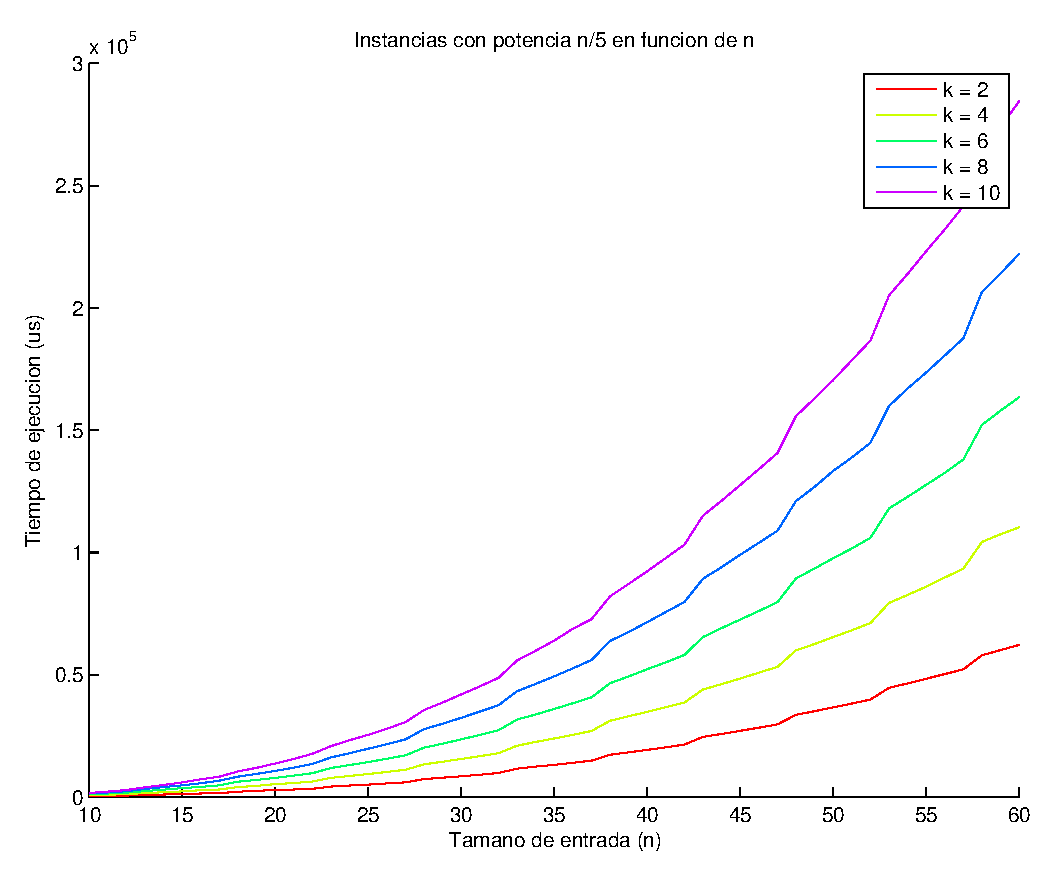
\includegraphics[width=\linewidth]{img/problema3/instancia_p_20p_varios_k.eps}
    \caption{Tiempo de ejecución, p(n) = $n/5$}\label{fig:problema3-k-20}
  \end{minipage}
  \hfill
  \begin{minipage}{0.5\linewidth}
    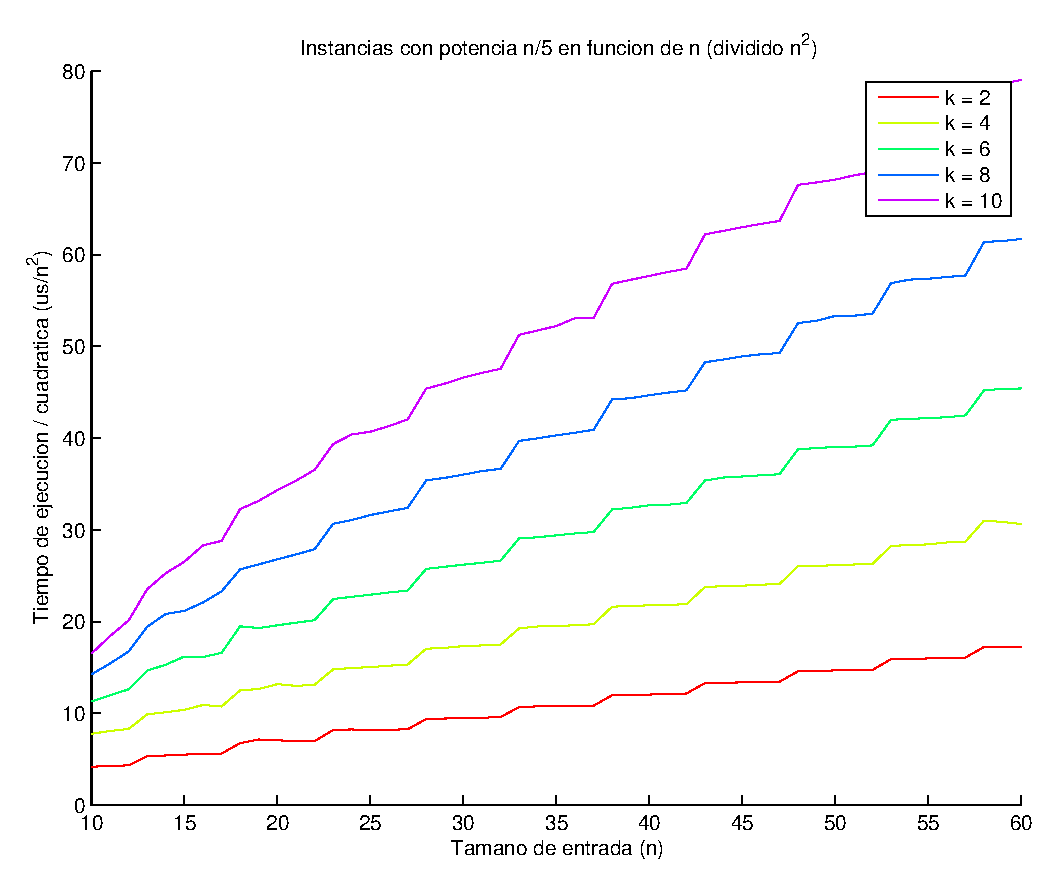
\includegraphics[width=\linewidth]{img/problema3/instancia_p_20p_varios_k_div_n2.eps}
    \caption{Idem, dividido por $n^2$}\label{fig:problema3-k-n2-20}
  \end{minipage}	
\end{figure}

En la figura \ref{fig:problema3-k-20} no podemos notar la complejidad temporal de la función. Por esto, dividimos por $n^2$ y plasmamos ese resultado en la figura \ref{fig:problema3-k-n2-20}. Sin embargo, en esta última figura tampoco podemos ver claramente la complejidad temporal. Por esta razón, decidimos analizar los ``saltos'' que pega la función. Luego de experimentación y búsqueda llegamos a la conclusión que esos saltos se relacionan con el cambio de potencia de los resortes. Por ejemplo entre para n entre 10 y 15 las potencias son de la siguiente manera: 2,2,2,3,3,3. Esto se debe a que 12/5 = 2.4 (y lo redondea para abajo) y 13/5 = 2.6 (que se redondea para arriba).

Una vez que entendimos estos saltos, llegamos a la conclusión que si tomamos los puntos donde pega los saltos la función y trazamos una recta $r$, la recta correspondiente al tiempo de ejecución va a tener una pendiente menor o igual a la pendiente de la recta $r$. Es decir, que comprobamos que por más que la potencia dependa del n la complejidad temporal también es lineal respecto de $T(N)/n^2$ que es lo mismo que decir que es cúbica respecto de n.

Finalmente, decidimos hacer un experimento más: utilizamos n distintos entre sí (pero fijos en cada caso) y variar el k. Una vez más p depende de n con la misma función anteriormente usada.

\begin{figure}[H]
  \begin{minipage}{0.5\linewidth}
    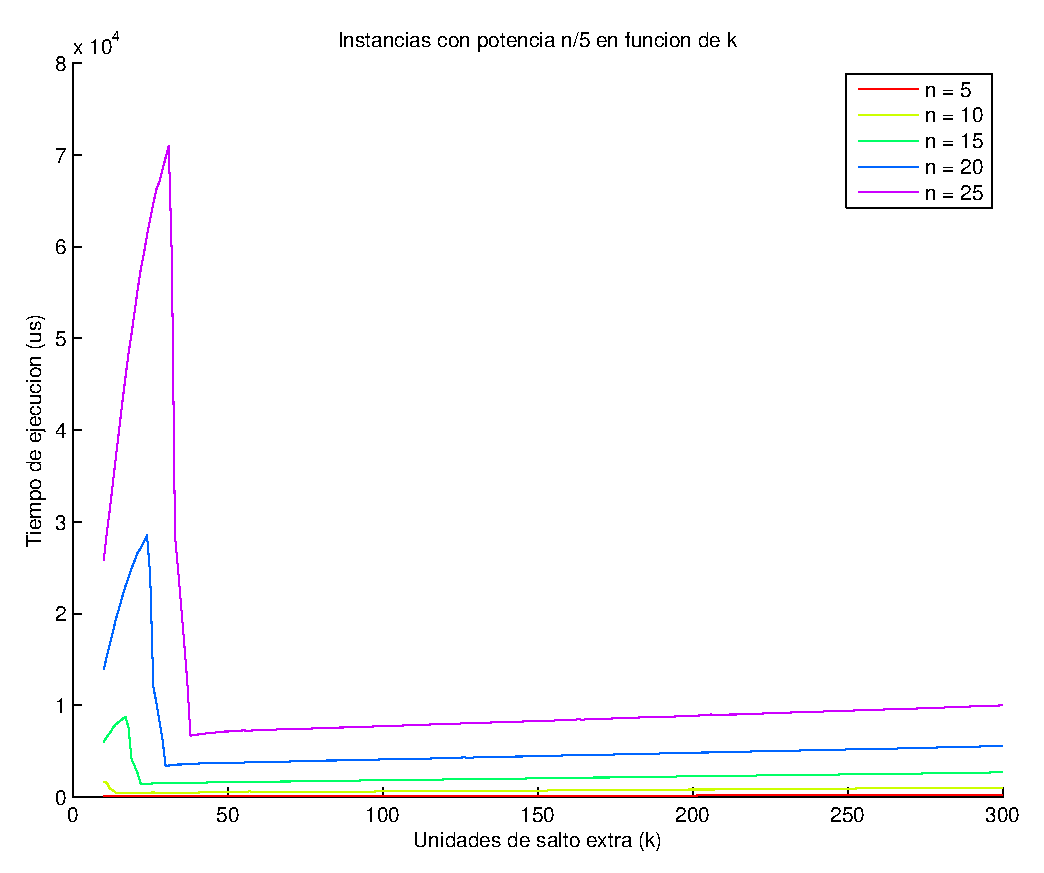
\includegraphics[width=\linewidth]{img/problema3/instancia_p_20p_varios_n.eps}
    \caption{Tiempo de ejecución, p(n) = $n/5$}\label{fig:problema3-n-20}
  \end{minipage}
  \hfill
  \begin{minipage}{0.5\linewidth}
    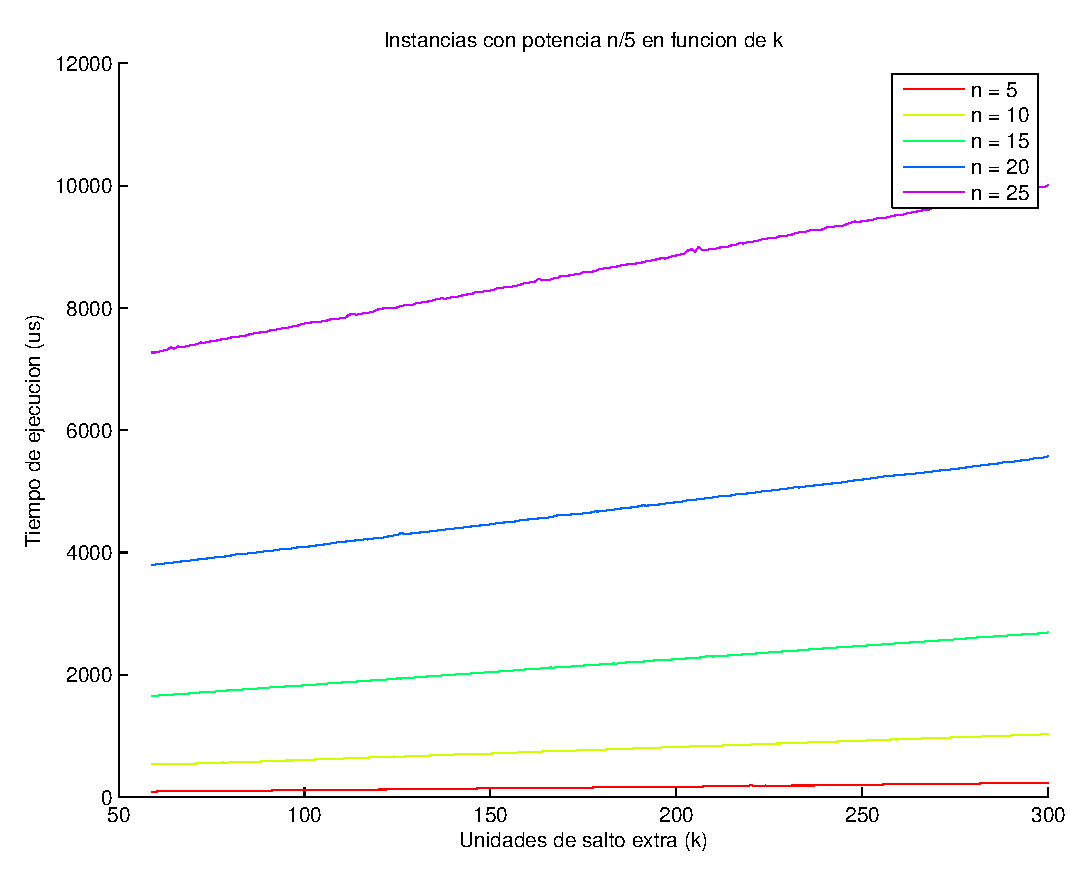
\includegraphics[width=\linewidth]{img/problema3/instancia_p_20p_varios_n_zoom.eps}
    \caption{Idem, con \emph{zoom}}\label{fig:problema3-n-n2-20}
  \end{minipage}
\end{figure}

En estos casos, una vez más podemos observar que cuando $k \geq 2*(n-1-p)$ resolver el problema es trivial. En estas figuras, está representado por la caída del tiempo de ejecución a partir de este punto. Cabe aclarar que si bien resolver el problema es trivial, al crecer el n cuesta más crear la matriz3D ya que la misma es más grande. En estos casos, la complejidad temporal de nuestro algoritmo es lineal respecto de k.

Para poder ver mejor esto último, realizamos \emph{zoom} a la figura a partir del momento de la caída, lo cual lo podemos ver en la figura \ref{fig:problema3-n-n2-20}. En esta figura, se ve claramente que la complejidad temporal de nuestro algoritmo es lineal respecto de k.

%TODO les parece poner un apendice con mas graficos o lo dejamos asi?

\subsection{Conclusión}
\label{problema2-resultados}
Si bien el problema tratado pareciera a primera vista admitir una solución en la forma de programación dinámica, el hecho de tener un recurso agotable en consideración no permite aplicar el principio de optimalidad. Es decir, es posible que en un camino óptimo se llegue a un casillero intermedio de forma subóptima (posiblemente para ahorrar unidades de salto extra).

De todas formas, el problema puede ser resuelto eficientemente una vez que se modela apropiadamente mediante grafos, utilizando el algorítmo de búsqueda BFS. En este caso, la representación de cada instancia no es tan trivial como asignar simplemente un nodo a cada casillero de la matriz, sino fue necesario desdoblar cada uno de ellos en $k$ nodos distintos. De esta forma, incorporamos dentro del grafo la información referente a las unidades de salto extra. Esto pone en evidencia que al modelar un problema, la representación de una instancia no necesariamente tiene que ser un mapeo directo o natural de los componentes del mismo.

Por otro lado, al haber dos variables $n$ y $k$ influyendo en el costo de la resolución del problema, la experimentación realizada resulta insuficiente para corroborar el resultado de complejidad temporal obtenido teóricamente. Logramos verificar empíricamente dentro del rango analizado que la función de costo muestra un comportamiento cúbico respecto a $n$ y lineal respecto a $k$. Sin embargo, esto no es suficiente para corroborar que $T(n,k) \in O(n^3 * k)$, ya que podría ser que $T(n,k) \in O(n^3 + k)$, mostrando el mismo comportamiento en la etapa de experimentación.

\newpage


%%%%%%%%%%%%%%%%%%%%%%%%%%%%%%%%%%%%%%%%%%%%%%%%%%%%%%%%%%%%%%%%%%%%%%%%%%%%%%%
%% Problema 3: Rompecolores                                                  %%
%%%%%%%%%%%%%%%%%%%%%%%%%%%%%%%%%%%%%%%%%%%%%%%%%%%%%%%%%%%%%%%%%%%%%%%%%%%%%%%

\section{Problema 3: Saltos en la Matrix}

\subsection{Descripción del problema}
\label{problema3-descripcion}
Este problema trata de un juego de cartas llamado \emph{Robanúmeros}. El mismo es un juego para dos jugadores. Al empezar el juego se cuenta con una secuencia de cartas, todas ellas boca arriba, cada carta tiene un valor numérico entero (puede ser positivo o negativo). Este juego se juega por turnos de forma alterna y en cada turno un jugador debe elegir un extremo de la secuencia de cartas y robar una cantidad de las mismas empezando desde ese extremo. Por ejemplo supongamos que la secuencia de cartas es la dada en la siguiente tabla:

\begin{tabular}{|c|c|c|c|c|}
\hline
2 & -3 & 7 & 8 & -10 \\
\hline
\end{tabular}

Dada esta secuencia, el primer jugador en jugar puede, por ejemplo, elegir el extremo derecho y robar 3 cartas, quedándose así con -10, 8 y 7. También podría elegir 4 cartas por el lado izquierdo y de esta forma se quedaría con 2, -3, 7 y 8. Sin embargo, el jugador no puede robar 2, -3 y 8, o -10, y -3.

En cada turno el jugador debe robar al menos una carta y al no quedar más, el jugador que obtenga el número más alto al sumar los valores de todas las cartas que robó es el ganador.

En este problema debemos diseñar un algoritmo que juegue a este juego de manera óptima. Este algoritmo debe estar pensado para jugar contra otro jugador que también juegue de forma óptima. La definición de que un jugador juegue de manera óptima significa que la diferencia de puntos obtenida a su favor sea la mayor diferencia que se puede obtener frente a un oponente que también juega de la misma forma ante cada situación que se le deje.

El algoritmo debe tener una complejidad temporal de peor caso de $O(n^3)$ donde $n$ es la cantidad de cartas en la secuencia inicial.

\subsubsection{Ejemplos y observaciones}



\subsection{Desarrollo de la solución}
\label{problema3-desarrollo}
Modelamos este problema de la siguiente manera:

$\bullet$ Un pueblo es un par ordenado (x,y).

$\bullet$ Una tubería es un par no ordenado de pueblos.

$\bullet$ Un conjunto de V pueblos y otro E de tuberías puede ser considerado un grafo, cuyo conjunto de nodos es V y su conjunto de aristas es E.

$\bullet$ El peso asociado a una arista (tubería) es igual a la distancia euclidiana entre los extremos (pueblos).

$\bullet$ Una central es un pueblo.

$\bullet$ Dado V un conjunto de pueblos y k la cantidad de centrales de gas, una solución es un conjunto $C \subseteq V$ de k pueblos y un grafo B(V,E), sea E el conjunto de tuberías que decidimos colocar para conectar los pueblos. Por ejemplo, si queremos conectar al pueblo 'a' y al pueblo 'b', agregamos al conjunto E la arista ('a','b'). El subonjunto C representa a los pueblos donde elegimos poner las centrales.  

$\bullet$ Dada una solución conformada por C y B(V,E), un pueblo $v \in V$ esta provisto de gas si existe un camino en B entre éste y un pueblo $c \in C$ ya que estos pueblos son los que tienen central distribuidora.

$\bullet$ Dada una solución C, B(V,E) decimos que la misma es factible si $(\forall v \in V)(\exists c \in C) \exists$ un camino entre v y c en B. 

$\bullet$ Queremos encontrar el C , B(V,E) tal que sea una solución óptima, minimizando la máxima arista.

Consideramos una solución, si cumple la aridad pedida. Una solución factible si cumple cierta condicion además de la aridad. Una solución optima es quien maximiza/minimiza cierta funcion entre todas las soluciones factibles, en este caso se busca minimizar la máxima arista.

Supongamos que tenemos el conjunto V que contiene a todos los pueblos. Sea G(V,E) un grafo completo donde el peso de las aristas es igual a la distancia euclidiana entre los pueblos. Para encontrar la solución óptima vamos a encontrar B(V,E) un bosque generador mínimo con k componentes conexas de G y C un conjunto que  contenga un pueblo de cada una de las componentes conexas de B.

Definiendo un bosque generador mínimo con k componentes conexas de G, como un grafo que cumple las siguientes condiciones:

$\bullet$Es un subgrafo generador de G. 

$\bullet$Es un bosque de k componentes conexas.

$\bullet$ Entre todos los subgrafos generador de G de k componentes conexas tiene la mínima suma de aristas.

Ahora presentaremos una idea de por este modelo efectivamente resuelve el problema. Luego lo vamos a demostrar formalmente. 

$\bullet$ Un bosque de k componentes conexas generador mínimo también minimiza la máxima arista.

$\bullet$ Dada una solución C, B(V,E), es factible $\Longleftrightarrow$ $(\forall D$ componente conexa de $B)((\exists v \in D) v \in C)$.  

$\bullet$ Dada una solución con i componentes conexas (siendo i $<$ k), existe una solución mejor o igual con i+1 componentes conexas.

Vamos a suponer que k $\leq$ n, ya que en el caso contrario la solución es trivial. Cada pueblo tiene una central y no se necesitan construir ninguna tubería.

\subsection{Complejidad temporal}
\label{problema3-complejidad}
En la figura que muestra el pseudocódigo de nuestro algoritmo situada arriba podemos ver que la complejidad de este algoritmo se representa con esta cuenta:

$O(n) + 2*O(1) + n*(2*O(1) + n*(2*O(1) +O(n) + 6*O(1)) + O(n)$

Por álgebra de órdenes esto se puede reducir a:

$O(2n+2) + n*(O(2) + n*(O(2) + O(n) + O (6)))$

$O(n) + n*(O(1) + n*(O(n+1)))$

$O(n) + n*(O(1) + O(n^2+n))$

$O(n) + n*(O(n^2 +n +1))$

$O(n) + n*O(n^2)$

$O(n^3+n)$

$O(n^3)$

Entonces podemos decir que la complejidad de nuestro algoritmo es $O(n^3)$, pero primero tenemos que demostrar que los algoritmos $escribirSalida$ y $buscarMinimo$ realmente tienen una complejidad lineal.

El algoritmo de $buscarMinimo$ es el siguiente

\begin{center}
 \begin{figure}[H]
  \begin{pseudo}
   \Procedure{buscarMinimo}{opt,i,j,iSiguiente,jSiguiente,minCantPuntos}
    \State $k \leftarrow 1$\Ode{1}
    \While{$k \leq j-1$} \hfill $n*O(1)$
      \If{$opt[i+k][j].cantPuntos < minCantPuntos$ }\Ode{1}
	\State $iSiguiente \leftarrow i+k$\Ode{1}
	\State $jSiguiente \leftarrow j$\Ode{1}
	\State $minCantPuntos \leftarrow opt[i+k][j].cantPuntos$\Ode{1}
      \EndIf
      \If{$opt[i][j-k].cantPuntos < mincantPuntos$}\Ode{1}
	\State $iSiguiente \leftarrow i$\Ode{1}
	\State $jSiguiente \leftarrow j-k$\Ode{1}
	\State $mincantPuntos \leftarrow opt[i][j-k].cantPuntos$\Ode{1}
      \EndIf
    \EndWhile
   \EndProcedure
  \end{pseudo}

 \end{figure}

\end{center}

La complejidad del algoritmo es:

$O(1) + n*(8*O(1))$

Por álgebra de órdenes:

$O(1) + O(8*n)$

$O(n)$

Ahora veamos que el algoritmo $escribirSalida$ también tiene complejidad lineal:

%Continuará


\subsection{Demostración de correctitud}
\label{problema3-demostracion}
Para demostrar que nuestra solución resuelve el problema propuesto tenemos que demostrar dos cosas. La primera es que la función recursiva que nosotros propusimos realmente determina los movimientos óptimos para realizar y la segunda es que la matriz que usamos para guardar las subsoluciones es completada correctamente.

Primero vamos a demostrar que la función recursiva determina las jugadas óptimas del juego. 

Para empezar recordemos lo que lo que el problema pide es jugar de una forma que maximice tu puntuación. Como al finalizar el juego no pueden quedar cartas sin robar, la suma de los valores de todas las cartas va a estar distribuida entre el jugador uno y el jugador dos, de esta forma:

$\sum_{i=0}^{n} c_i = \sum_{j \in A} c_j + \sum_{k \in B} c_k$

Donde A es el conjunto de cartas que robó el jugador uno y B es el conjunto de cartas que robó el jugador dos.

Por lo tanto mientras más chico sea el valor de la suma de los valores del conjunto B, el valor del conjunto A va a crecer, y viceversa, ya que se da la siguiente igualdad:

$\sum_{i=0}^{n} c_i  - \sum_{j \in B} c_j= \sum_{k \in A} c_k$

Supongamos que somos el jugador uno. Lo que el problema pide es que juguemos de forma óptima, por lo tanto debemos maximizar nuestra puntuación. Maximizar nuestra puntuación es maximizar el valor de la suma de los elementos de A, y  por lo que acabamos de ver esto es lo mismo que minimizar la suma de los elementos de B, que representa la puntuación del jugador dos.

Recordemos que nuestra función recursiva es la siguiente:

$opt(i,i) = c_i$ \\
$opt(i,j) = \sum cartas - min(opt(i+1, j), ..., opt(j,j), opt(i, j-1), ... ,opt(i,i), 0)$

Por lo dicho anteriormente demostrar que nuestra función resuelve el problema es lo mismo que demostrar que nuestra función minimiza el puntaje del jugador contrario.

Vamos a demostrar esto por inducción en las cartas restantes, que en este caso son $j-i+1$. La propiedad que queremos demostrar es la siguiente:

$P(i,j) : (\forall i,j, 0 \leq i \leq j < n)opt(i,j)$ maximiza nuestro puntaje para las cartas desde $c_i$ hasta $c_j$

Primero analicemos el caso base:

$opt(i,i) = c_i$

Queremos ver que se cumple $P(i,i)$.

Este caso significa que sólo queda una carta. Como el juego nos obliga a, de ser posible, robar al menos una carta por turno, la única opción posible es robar esta carta. Como es la última opción, también es la opción óptima, por lo tanto se cumple $P(i,i)$.

Ahora analicemos el caso recursivo:

$opt(i,j) = \sum cartas - min(opt(i+1, j), ..., opt(j,j), opt(i, j-1), ... ,opt(i,i), 0)$

Tenemos que realizar el paso inductivo, esto significa que tenemos que probar que $P(i,j)$ seguro vale si vale $P(i',j')$ para todas las subsecuencias de cartas que $opt(i,j)$ utiliza, osea, para probar $P(i,j)$ queremos ver que:

$[(\forall i',j',(( i < i' \wedge j = j') \vee (i' = i \wedge j' < j))) P(i',j')]  \implies P(i,j)$

\textbf{HI:} $((\forall i',j',(( i < i' \wedge j = j') \vee (i' = i \wedge j' < j))) P(i',j'))$

Para demostrar esto vamos a dar como válida la hipótesis inductiva y a partir de eso probar que vale $P(i,j)$.

En este caso quedan $j-i+1$ cartas, tenemos que demostrar que $opt(i,j)$ toma la decisión que minimiza el puntaje del jugador contrario. Como el problema nos dice que tenemos que asumir que el jugador contrario también juega de forma óptima, entonces su puntaje también estará determinado por la función $opt$.

Lo que la función debe determinar es, de las posibles instancias del juego que se pueden generar luego de jugar nuestro turno, la que minimiza la función de $opt$ ya que el puntaje del jugador contrario será el resultado de aplicar $opt$ a la instancia que quede. Y por hipótesis inductiva sabemos que al aplicar $opt$ a dicha instancia se obtendrá un resultado óptimo.

Como sólo se pueden robar cartas de uno de los dos extremos las posibles instancias son las siguientes: Si se roba una carta comenzando de la izquierda la instancia generada será de $(i+1,j)$, si se roban 2, de $(i+2,j)$ y se se roban $j-i$, de $(j,j)$. De esta misma forma si se roba una carta empezando de la derecha quedará una instancia de $(i,j-1)$ y si se roban $j-i$ cartas, la instancia sera de $(i,i)$.

Pero queda una instancia más por analizar, la de levantar todas las cartas posibles (no importa de cual extremo). En ese caso se generará una instancia $(0,0)$.

Por lo tanto el mínimo que debemos hallar es el siguiente:

$min(opt(i+1,j), ... , opt(j,j), opt(i,j-1), ... , opt(i,i), 0)$

Y la puntuación óptima se determina por la cuenta:

$\sum cartas - min(opt(i+1,j), ... , opt(j,j), opt(i,j-1), ... , opt(i,i), 0)$

Por lo tanto, si asumimos que se cumple nuestra hipótesis inductiva, nuestra función $opt$ minimiza el puntaje del jugador contrario. Osea que realmente determina nuestra puntuación óptima y el movimiento a realizar para obtenerla, que es lo que el problema pide.

Lo que queda mostrar es que completamos la matriz de forma correcta. Como cada casilla de la matriz es un subproblema y para resolver cada subproblema usamos subproblemas mas chicos, tenemos que mostrar que a la hora de completar una casilla siempre tenemos completas las casillas de los subproblemas que se necesitan.

La matriz, tal y como dijimos en el desarrollo, se completa de arriba a abajo y de izquierda a derecha.

Entonces, supongamos que queremos llenar la casilla $opt[i][j]$. Como la matriz se llena de abajo hacia arriba, a la hora de llenar esta casilla ya van a estar llenas las casillas $opt[i][j']$ donde $j < j'$. Y como la matriz se llena de izquierda a derecha, a la hora de completar esta casilla ya van a estar completas las casillas $opt[i'][j]$, donde $i' < i$.

Además, como dijimos en el desarrollo para llenar una casilla $opt[i][j]$ se necesita observar los valores de las casillas que están a la izquierda de la ésta y las que están abajo. Como se muestra en la Figura 1.

Osea que las casillas necesarias son $opt[i'][j]$, donde $i' < i$ y $opt[i][j']$ donde $j < j'$. Estas son las mismas casillas que ya dijimos que iban a estar completas a la hora de completar $opt[i][j]$. Por lo tanto al completar $opt[i][j]$ casilla van a estar previamente completadas las casillas necesarias para hacerlo, por lo tanto nuestra matriz se llena correctamente.

\subsection{Experimentación}
\label{problema3-experimentacion}
En esta sección, vamos a comprobar empíricamente que nuestro algoritmo tiene una complejidad temporal cúbica respecto de n, y lineal respecto de k.

En un primer caso, utilizamos instancias donde cada casillero tiene una potencia en función de n: p(n) = $n/5$. Una vez más, utilizamos k distintos entre sí, pero fijos en cada caso. Probamos con distintos $n$ y obtuvimos el resultado que se puede observar en las figuras debajo.

\begin{figure}[H]
  \begin{minipage}{0.5\linewidth}
    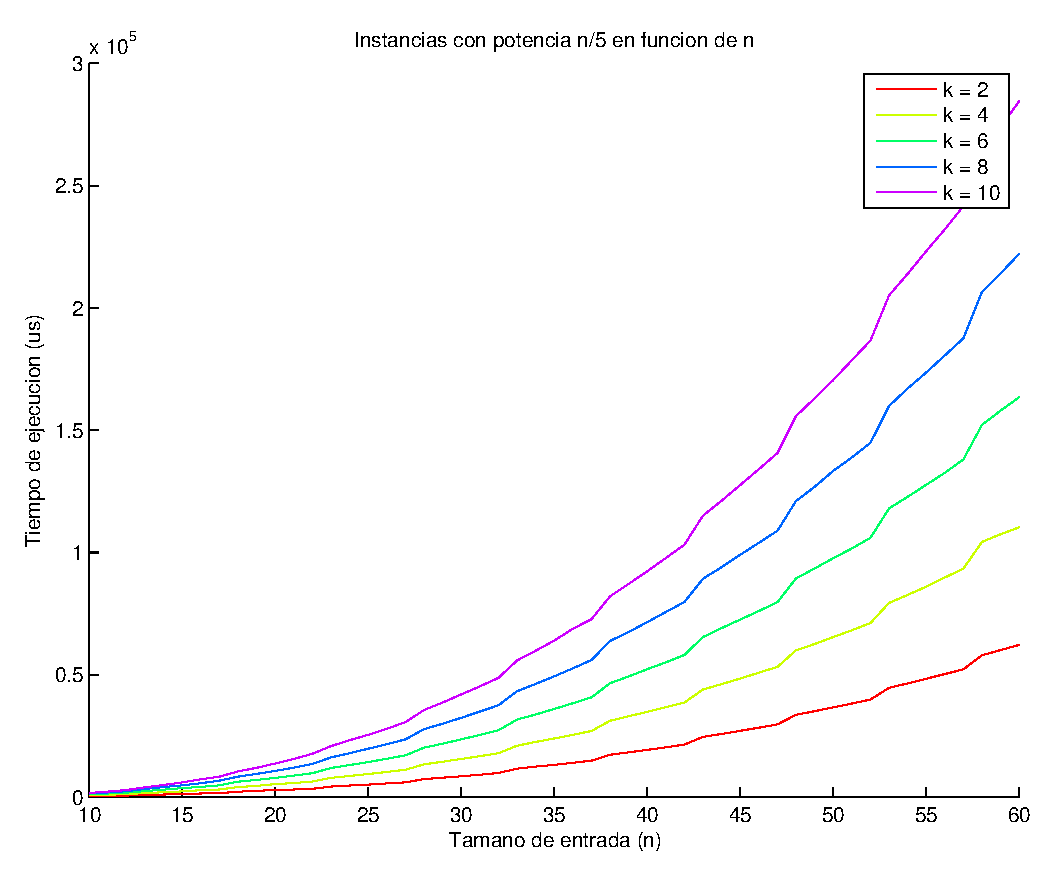
\includegraphics[width=\linewidth]{img/problema3/instancia_p_20p_varios_k.eps}
    \caption{Tiempo de ejecución, p(n) = $n/5$}\label{fig:problema3-k-20}
  \end{minipage}
  \hfill
  \begin{minipage}{0.5\linewidth}
    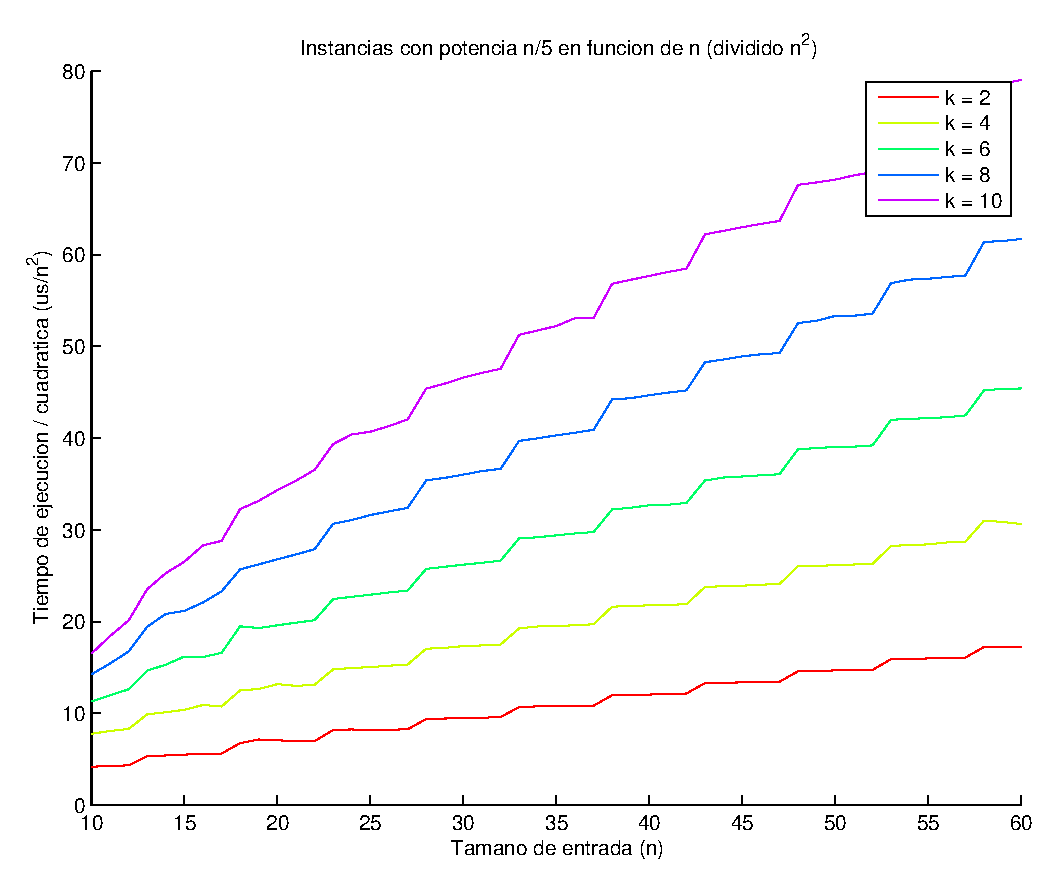
\includegraphics[width=\linewidth]{img/problema3/instancia_p_20p_varios_k_div_n2.eps}
    \caption{Idem, dividido por $n^2$}\label{fig:problema3-k-n2-20}
  \end{minipage}	
\end{figure}

En la figura \ref{fig:problema3-k-20} no podemos notar la complejidad temporal de la función. Por esto, dividimos por $n^2$ y plasmamos ese resultado en la figura \ref{fig:problema3-k-n2-20}. Sin embargo, en esta última figura tampoco podemos ver claramente la complejidad temporal. Por esta razón, decidimos analizar los ``saltos'' que pega la función. Luego de experimentación y búsqueda llegamos a la conclusión que esos saltos se relacionan con el cambio de potencia de los resortes. Por ejemplo entre para n entre 10 y 15 las potencias son de la siguiente manera: 2,2,2,3,3,3. Esto se debe a que 12/5 = 2.4 (y lo redondea para abajo) y 13/5 = 2.6 (que se redondea para arriba).

Una vez que entendimos estos saltos, llegamos a la conclusión que si tomamos los puntos donde pega los saltos la función y trazamos una recta $r$, la recta correspondiente al tiempo de ejecución va a tener una pendiente menor o igual a la pendiente de la recta $r$. Es decir, que comprobamos que por más que la potencia dependa del n la complejidad temporal también es lineal respecto de $T(N)/n^2$ que es lo mismo que decir que es cúbica respecto de n.

Finalmente, decidimos hacer un experimento más: utilizamos n distintos entre sí (pero fijos en cada caso) y variar el k. Una vez más p depende de n con la misma función anteriormente usada.

\begin{figure}[H]
  \begin{minipage}{0.5\linewidth}
    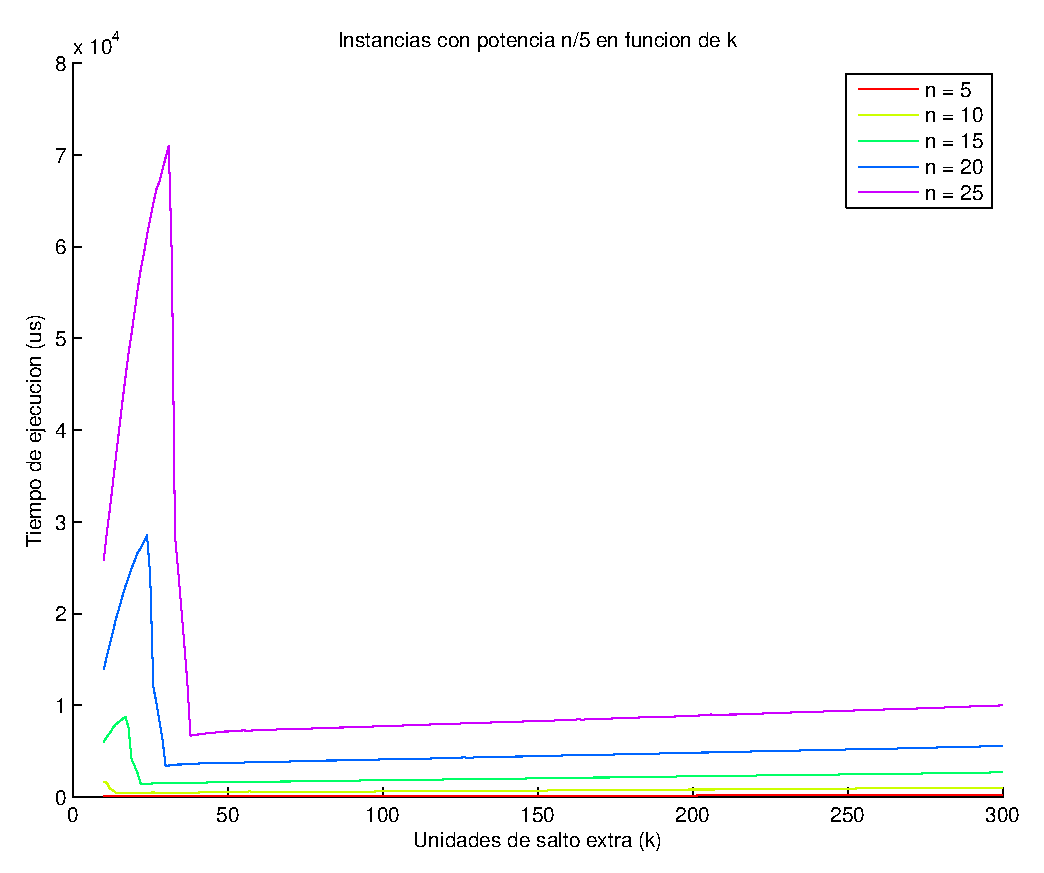
\includegraphics[width=\linewidth]{img/problema3/instancia_p_20p_varios_n.eps}
    \caption{Tiempo de ejecución, p(n) = $n/5$}\label{fig:problema3-n-20}
  \end{minipage}
  \hfill
  \begin{minipage}{0.5\linewidth}
    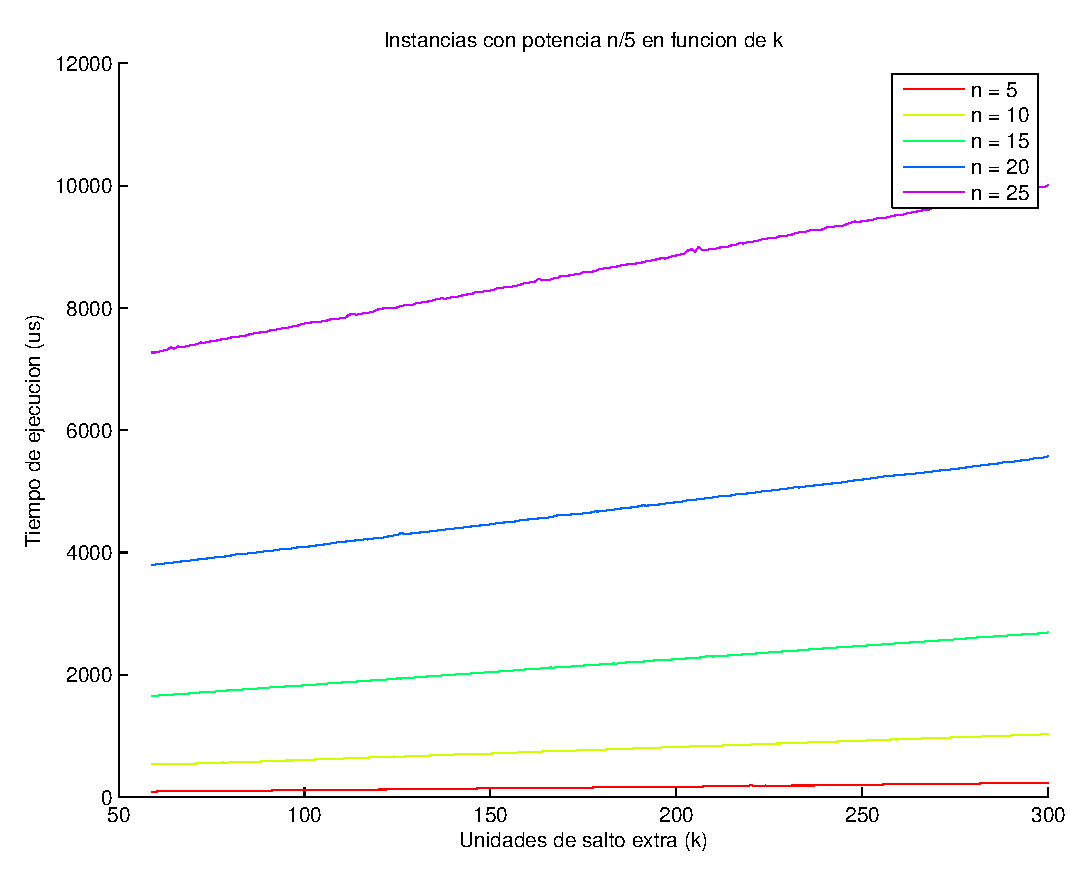
\includegraphics[width=\linewidth]{img/problema3/instancia_p_20p_varios_n_zoom.eps}
    \caption{Idem, con \emph{zoom}}\label{fig:problema3-n-n2-20}
  \end{minipage}
\end{figure}

En estos casos, una vez más podemos observar que cuando $k \geq 2*(n-1-p)$ resolver el problema es trivial. En estas figuras, está representado por la caída del tiempo de ejecución a partir de este punto. Cabe aclarar que si bien resolver el problema es trivial, al crecer el n cuesta más crear la matriz3D ya que la misma es más grande. En estos casos, la complejidad temporal de nuestro algoritmo es lineal respecto de k.

Para poder ver mejor esto último, realizamos \emph{zoom} a la figura a partir del momento de la caída, lo cual lo podemos ver en la figura \ref{fig:problema3-n-n2-20}. En esta figura, se ve claramente que la complejidad temporal de nuestro algoritmo es lineal respecto de k.

%TODO les parece poner un apendice con mas graficos o lo dejamos asi?

\subsection{Conclusión}
\label{problema3-resultados}
Si bien el problema tratado pareciera a primera vista admitir una solución en la forma de programación dinámica, el hecho de tener un recurso agotable en consideración no permite aplicar el principio de optimalidad. Es decir, es posible que en un camino óptimo se llegue a un casillero intermedio de forma subóptima (posiblemente para ahorrar unidades de salto extra).

De todas formas, el problema puede ser resuelto eficientemente una vez que se modela apropiadamente mediante grafos, utilizando el algorítmo de búsqueda BFS. En este caso, la representación de cada instancia no es tan trivial como asignar simplemente un nodo a cada casillero de la matriz, sino fue necesario desdoblar cada uno de ellos en $k$ nodos distintos. De esta forma, incorporamos dentro del grafo la información referente a las unidades de salto extra. Esto pone en evidencia que al modelar un problema, la representación de una instancia no necesariamente tiene que ser un mapeo directo o natural de los componentes del mismo.

Por otro lado, al haber dos variables $n$ y $k$ influyendo en el costo de la resolución del problema, la experimentación realizada resulta insuficiente para corroborar el resultado de complejidad temporal obtenido teóricamente. Logramos verificar empíricamente dentro del rango analizado que la función de costo muestra un comportamiento cúbico respecto a $n$ y lineal respecto a $k$. Sin embargo, esto no es suficiente para corroborar que $T(n,k) \in O(n^3 * k)$, ya que podría ser que $T(n,k) \in O(n^3 + k)$, mostrando el mismo comportamiento en la etapa de experimentación.

\newpage


%%%%%%%%%%%%%%%%%%%%%%%%%%%%%%%%%%%%%%%%%%%%%%%%%%%%%%%%%%%%%%%%%%%%%%%%%%%%%%%
%% Apéndices                                                                 %%
%%%%%%%%%%%%%%%%%%%%%%%%%%%%%%%%%%%%%%%%%%%%%%%%%%%%%%%%%%%%%%%%%%%%%%%%%%%%%%%

\begin{appendices}

\section{Código fuente del problema 1}
\label{problema1-codigo}

\verbatiminput{./codigo/problema1.cpp}

\newpage


\section{Código fuente del problema 2}
\label{problema2-codigo}
\verbatiminput{./codigo/problema2.cpp}

\newpage


\section{Código fuente del problema 3}
\label{problema3-codigo}
\verbatiminput{./codigo/problema3.cpp}


\end{appendices}

\end{document}